%!TEX root = ../dokumentation.tex

\chapter{Technische Grundlagen}
In dem dritten Kapitel dieser wissenschaftlichen Arbeit werden einerseits die Kriterien erläutert, die erfüllt sein müssen, dass das Projekt nach dem Abschluss als erfolgreich oder nicht erfolgreich bezeichnet werden kann. Die Auswertung mit dem Bezug auf die Kriterienformulierung wird in Kapitel \ref{evaluation} stattfinden.

Andererseits wird die zu verwendende Bibliothek vorgestellt und evaluiert. Dabei werden die Eigenschaften, Vor- und Nachteile dieser aufgeschlüsselt und diese anhand von Beispielen erläutert.

% Die zu verwendende Bibliothek vorgestellt und evaluiert. Dabei werden Eigenschaften, Vor- und Nachteile dieser aufgeschlüsselt.

\section{Kriterienformulierung}\label{kriterienformulierung}
Nachdem in Kapitel \ref{zweck_und_ziel} bereits auf das Ziel der wissenschaftlichen Arbeit eingegangen wurde, in Kapitel \ref{game_types} bis \ref{evaluation_func} das benötigte Grundwissen vermittelt wurde, das für das Verständnis der Umsetzung notwending ist, werden nun die Merkmale und Eigenschaften dargelegt, die erfüllt werden sollen.

Grundlegend wird eine Künstliche Intelligenz für das Spiel Schach entwickelt worden sein. Der Fokus dieser Implementierung liegt dabei die in Kapitel \ref{theoretische_hintergründe} vorgestellten Algorithmen und deren Wirkungsweise zu demonstrieren.

Dabei wird das Programm nach Beendigung der Implementierung darauf ausgelegt sein, ein Schachspiel zwischen einem Spieler und einer KI über eine Konsole durchzuführen. Die dazu zu entwickelnde Künstliche Intelligenz benötigt dafür den Elo Wert eines Amateurs. Der Elo Wert ist benannt nach seinem Erfinder Professor Arpad Elo, der ein Bewertungssystem entwickelt hat, das ein Gradmesser für die Spielstärke eines Schachspielers ist.\cite{E.V.} 

Jeder Schachspieler erhält einen Elo-Wert zugewiesen, der Aufschluss über die Stärke eines Spielers gibt. Umso höher der Elo-Wert eines Spielers, desto besser ist dieser. Sobald zwei Konkurrenten gegeneinander antreten lässt sich aus den ihn zugewiesenen Elo-Zahlen, mittels des Erwartungswertes, eine Punktezahl errechnen, die Aufschluss über den Ausgang des Spiels gibt. 
Berechnet wird der Erwartungswert($E_{A}$) des Punktestands für Spieler A vor einem Spiel, indem dieser aus der bisherigen Elo-Zahl von Spieler A($R_{A}$) und Spieler B($R_{B}$) evaluiert wird.

\begin{equation}
\begin{aligned}
E_{A} = \frac{1}{1 + 10^{({R_{B} - R_{A}})/400}}
\end{aligned}
\end{equation}

Nachdem ein Spiel beendet wurde, wird die Diskrepanz zwischen dem zuvor berechneten Erwartungswert und dem Ergebnis ermittelt und auf dieser Grundlage die Elo-Werte der Spieler angepasst. Hierbei ergibt sich der neue Elo-Wert($R'_{A}$) von Spieler A aus dem alten Elo-Wert, einem Faktor $K$, der gewichtet wie stark sich neu erzielte Ergebnisse auswirken, dem Ergebnispunktestand des Spiels ($S_{A}$) und dem Erwartungswert. Der Faktor $K$ wird an die Stärke eines Spielers angepasst.

\begin{equation}
\begin{aligned}
R'_{A} = R_{A} + K \cdot (S_{A} - E_{A})
\cite{Elo1987}
\end{aligned}
\end{equation}

Zur Ermittlung eines Elo-Werts eines neuen Spielers wird dessen Wert geschätzt. In dem \href{https://www.fide.com/fide/handbook.html?id=197&view=article}{Bewertungssystem}, das in den Statuten der Fédération Internationale des Échecs verwendet wird, ist definiert, dass ein Amateurspieler einen Elo Wert von 1000 hat. Alle Spieler mit einem geringeren Wert werden nicht gelistet.\cite{FIDE2017}

Durch die Entwicklung von Evaluierungsfunktionen wird die Schach KI die Möglichkeit besitzen die besten Züge für eine spezielle Spielsituation ermitteln zu können. Dabei wird eine Historie integriert sein, die es ermöglicht auf einer Basis von vergangenen Spielen Zügen einen Wert zuzuweisen und daraus einen optimalen auszuwählen. Ebenfalls wird die Schach KI anhand der Anzahl und Wichtigkeit attackierter Steine, sowie des insgesamten Wertes aller sich auf dem Spielfeld befindlichen Steine, einen guten Zug auszuwählen.

Die Benutzinteraktionen wird durch Verwendung von \acs{ASCII} (American Standard Code for Information Interchange) Zeichen in einer Konsole visualisiert werden. Zukünftige Erweiterungen des Programms werden durch eine gute Dokumentation des Codes garantiert werden. Ebenfalls wird nach der erfolgreichen Beendigung dieser Arbeit ein beliebig erweiterbares Grundgerüst für eine Schach-KI vorliegen.

% Wie kann überprüft werden, ob das Porjekt erfolgreich verlaufen ist?

\iffalse
2. Entwicklung einer KI für das Schach-Spiel

   Das Schachspiel ist in der westlichen Welt das am weitesten verbreitete Brett-Spiel.  Ziel der Studienarbeit
   ist die Entwicklung eines Schachprogramms.  Das wesentliche Ziel bei der Entwicklung dieses Programms
   besteht darin, die Wirkungsweise der im Rahmen der KI-Vorlesung vorgestellten Algorithmen zu demonstrieren.
   Insbesondere wird es wichtig sein, zur Evaluation einer Stellung eine gute Heuristik
   zu entwickeln.  Bei der Entwicklung dieser Heuristik sollen Techniken des Machine-Learnings eingesetzt
   werden.

Anforderungen:
	Keine hohe ELO Zahl
	klarer/cleaner Code
	Techniken aus Vorlesung erkennbar
	Tagebuch führen
	Regelmäßige Treffen
	ASCII Ausgabe
	Grundgerüst aufgesetzt
	Einfacher Evaluierungsprozess
\fi


    \section{Python-Chess Evaluierung}\label{python-chess-evaluierung}

In diesem Notebook wird die ``python-chess-library``, oder auch ``chess
core`` genannt, Bibliothek evaluiert. Der ``chess core`` soll Funktionen
zum Erstellen des Schachbretts, berechnen der erlaubten/möglichen Züge,
durchführen der Züge etc. bereitstellen.

Dabei wird jede notwendige Funktion getestet und dessen Realisierung
dokumentiert. Alle notwendigen Funktionen sind folgend gelistet.

\begin{itemize}
\tightlist
\item
  Schachbrett erstellen
\item
  Schachbrett als ASCII ausgeben
\item
  Züge auf dem Schachbrett ziehen
\item
  Erlaubte Züge berechnen
\item
  Auf Schach/Schachmatt prüfen
\item
  Testen, ob Rochade, En Passant als erlaubte Züge gelistet werden
\item
  \emph{(Optional)} Schachbrett als SVG in JupyterNotebook ausgeben
\item
  \emph{(Optional)} Möglichkeiten evaluieren, Schachbrett je nach
  Positionierungen eindeutig identifizierbar in CSV zu schreiben
\end{itemize}

Des Weiteren werden folgende Aktionen/Berechnungen auf deren
Umsetzbarkeit getestet. Dabei wird herausgefunden werden was nötig ist,
um die aufgelisteten Aktionen mit der Bibliothek durchzuführen.

\begin{itemize}
\tightlist
\item
  Berechnen \& Ausgeben erlaubter Züge für eine spezielle Figur
\item
  Abwechselnder User \& KI Input auf demselben Board
\item
  Berechnen des Wertes des Schachbretts und der attackierten Figuren
\item
  Speichern von Zügen/Entwicklung eines Schachbretts inklusive
  Sieg/Niederlagen als CSV-Datei
\end{itemize}

\subsection{Vorraussetzungen}\label{vorraussetzungen}

Folgend werden die allgemeinen Vorraussetzungen für die Verwendung und
Installation der ``python-chess-library`` erläutert.

\begin{itemize}
\tightlist
\item
  Python 3 Da die zu verwendende Bibliothek auf Python 3 basiert muss
  diese Version auf dem auszuführenden Computer vorhanden sein.

  \begin{itemize}
  \tightlist
  \item
    \href{https://wsvincent.com/install-python3-mac/}{macOS}
  \item
    \href{https://docs.python-guide.org/starting/install3/linux/}{Linux}
  \item
    \href{https://realpython.com/installing-python/}{Win}
  \end{itemize}
\item
  Jupyter Notebooks Damit die aufgeführten Scripts direkt im Browser
  ausgeführt werden können haben sich die Autoren dieser Arbeit darauf
  verständigt Jupyter Notebook zu nutzen. Dabei bietet diese Applikation
  den Vorteil, dass Code und Dokumente live geteilt werden können und
  der entwickelte Code sofort ausgeführt werden kann. Ebenfalls bietet
  Jupyter Notebook die Möglichkeit unter Anderem Daten zu visualisieren.

  \begin{itemize}
  \tightlist
  \item
    \href{https://jupyter.org/install}{Installationsanleitung}
  \end{itemize}
\item
  ``python-chess-library``

  \begin{itemize}
  \tightlist
  \item
    \texttt{pip\ install\ python-chess} Im weiteren Verlauf dieses
    Notebooks werden zusätzliche Module, wie beispielsweise Pandas,
    genutzt, die ebenfalls auf dem auszuführenden Rechner installiert
    sein müssen.
  \end{itemize}
\end{itemize}

\subsection{FEN-Notation}\label{FEN-Notation}

Die ``FEN`` Notation, oder auch Forsyth-Edwars-Notation, ist eine gekürzte Form der Darstellung des Spielbretts, wobei das Spielbrett dennoch eindeutig identifizierbar bleibt. Dabei wird neben der Figurenstellung, dem Zugrecht, das Rochaderecht, ein möglicher En-passant-Schlag und den bereits gespielten Halbzügen seit dem letzten Bauernzug, oder einem Schlag, die Nummer des nächsten Zugs angegeben.\cite{FEN2019}

Diese Notation ist ein essenzieller Bestandteil der einzuführenden Python Bibliothek. Folgend ist ein Beispiel gegeben, das die Startposition eines neuen Schachspiels widerspiegelt.

\begin{Verbatim}[commandchars=\\\{\}]
rnbqkbnr/pppppppp/8/8/8/8/PPPPPPPP/RNBQKBNR w KQkq - 0 1
\end{Verbatim}

Die Zeichenkette bis zum ersten Leerzeichen beschreibt die Positionen der schwarzen und weißen Steine. Hierbei beschreiben die Großbuchstaben die weißen und die Kleinbuchstaben die schwarzen Figuren. Die Zeichenketten zwischen den Schrägstichen beschreiben jeweils eine Zeile des Schachbretts. Die Bedeutungen der unterschiedlichen Buchstaben wird im folgenden Kapitel \ref{erstellen-eines-schachbretts-und-ausgeben-als-ascii} erläutert. Die Zahlen, die in der Positionsangabe verwendet werden, beschreiben die Anzahl der Felder, auf der sich kein Stein befindet.

Das Zeichen nach den Positionen beschreibt mit ``w`` oder ``b`` das Zugrecht und wird von dem Rochaderecht gefolgt. Da in dieser Situation kein En-passant-Schlag möglich ist, ist für diesen Parameter das Zeichen ``-``angegeben.

Der Wert der bereits gespielten Halbzüge seit dem letzten Bauernzug, oder Schlag, beträgt in diesem Fall ``0``, da noch kein Zug unternommen wurde. Die Nummer des nächsten Zugs ist bei ``1``, da es sich um eine Startposition handelt.

    \subsection{Erstellen eines Schachbretts und ausgeben als
ASCII}\label{erstellen-eines-schachbretts-und-ausgeben-als-ascii}

Folgend wird die Python-Chess-Library eingebunden, die für den
weiteren Verlauf der Evaluierung und Implementierung benötigt wird.

    \begin{Verbatim}[commandchars=\\\{\}]
{\color{incolor}In [{\color{incolor}1}]:} \PY{k+kn}{import} \PY{n+nn}{chess}
\end{Verbatim}


    Das unten einzusehende Code Snippet zeigt, wie ein neues Schachbrett mit
standardmäßigen Positionierungen der Figuren erstellt werden kann. Dies
ist umzusetzen durch den Aufruf der \texttt{chess.Board()} Funktion und
das Speicherns der Rückgabe dieser Funktion in einer \texttt{board}
Variable. Dieses \texttt{board} beinhaltet die Positionierungen aller
Figuren und kann mittels der python-eigenen \texttt{print()} Funktion
als ASCII Code ausgegeben werden, wie unten einzusehen ist. Zuletzt wird
noch die Möglichkeit aufgezeigt, die auf einem spezifizierten Feld
befindliche Figur auszulesen. Dieses Feld wird dabei über das Datenfeld
\texttt{chess.B1} aufgerufen.

    \begin{Verbatim}[commandchars=\\\{\}]
{\color{incolor}In [{\color{incolor}2}]:} \PY{n}{board} \PY{o}{=} \PY{n}{chess}\PY{o}{.}\PY{n}{Board}\PY{p}{(}\PY{p}{)}
            
        \PY{n+nb}{print} \PY{p}{(}\PY{l+s+s2}{\PYZdq{}}\PY{l+s+se}{\PYZbs{}n}\PY{l+s+s2}{Board:}\PY{l+s+s2}{\PYZdq{}}\PY{p}{)}
        \PY{n+nb}{print} \PY{p}{(}\PY{n}{board}\PY{p}{)}
        
        \PY{n+nb}{print} \PY{p}{(}\PY{l+s+s2}{\PYZdq{}}\PY{l+s+se}{\PYZbs{}n}\PY{l+s+s2}{Piece at B1:}\PY{l+s+s2}{\PYZdq{}}\PY{p}{)}
        \PY{n+nb}{print} \PY{p}{(}\PY{n}{board}\PY{o}{.}\PY{n}{piece\PYZus{}at}\PY{p}{(}\PY{n}{chess}\PY{o}{.}\PY{n}{B1}\PY{p}{)}\PY{p}{)}
\end{Verbatim}


    \begin{Verbatim}[commandchars=\\\{\}]

Board:
r n b q k b n r
p p p p p p p p
. . . . . . . .
. . . . . . . .
. . . . . . . .
. . . . . . . .
P P P P P P P P
R N B Q K B N R

Piece at B1:
N

    \end{Verbatim}

    Dabei ist einzusehen, dass die Figuren durch einen Buchstaben abgekürzt
werden. Figuren des Spielers der schwarzen Steine werden als Kleinbuchstaben
dargestellt, Figuren des Spielers der weißen Steine als äquivalente
Großbuchstaben. Leere Felder werden mit einem Punkt dargestellt. Aus
folgender Liste kann die Zuordnung der Buchstaben zu den Schachfiguren
entnommen werden:

\begin{itemize}
\tightlist
\item
  p/P: Pawn / Bauer
\item
  r/R: Rook / Turm
\item
  n/N: Knight / Springer
\item
  b/B: Bishop / Läufer
\item
  q/Q: Queen / Dame
\item
  k/K: King / König
\end{itemize}

    Die Zuordnung der Felder findet mittels einer Kombination aus einem
Buchstaben und einer Zahl statt. Die Buchstaben A-H geben dabei die
vertikalen Reihe an, die Zahlen 1-8 die horizontalen Reihen. Jedem Feld
wird eine namensäquivalente Variable in der statischen Klasse ``chess``
zugeordnet, wie beispielhaft in Zeile 16 im oberen Code Snippet erkannt
werden kann.

    \subsection{Alternierende Eingaben von Nutzer \&
KI}\label{alternierende-eingaben-von-nutzer-ki}

Damit ein Schachspiel zustande kommen kann, ist es zwingend
erforderlich, dass Nutzer und KI abwechselnd Züge auswählen und zum
Board ``pushen`` können. Dafür muss zunächst überprüft werden, welcher
Spieler an der Reihe ist und dieser muss einen Zug auswählen können, der
daraufhin von dem Schachbrett übernommen wird. Auf diesem Schachbrett
kann dann der nächste Spieler seinen Zug auswählen.

Bei der \emph{``python-chess``} Bibliothek kann der zu agierende Spieler
über die \texttt{board.turn} Variable ermittelt werden. Diese steht auf
\texttt{True} wenn Spieler 1 an der Reihe ist und auf \texttt{False},
wenn Spieler 2 den nächsten Zug machen muss. Beim Ausführen einer
\texttt{push} Operation auf dem \texttt{board}, wechselt die Variable
automatisch ihren Wert.

Damit das Spiel erkennt, wann dieses vorbei ist, bietet die Bibliothek
die \texttt{board.is\_game\_over()} Funktion. Diese gibt den Wert
\texttt{True} zurück, falls das Spiel auf Grund eines Schachmatts oder
anderer spielbeendender Umstände vorbei ist.

Um alle möglichen Züge ausgeben zu können, bietet die verwendete
Bibliothek die Funktion \texttt{board.legal\_moves}. Diese gibt alle
gültigen Züge nach \emph{chess960} Standard aus. Dabei werden nur die
Züge ausgegeben, die zum einen vom aktuellen Schachbrett aus
durchführbar sind und zum anderen nicht zu einer unmittelbaren
Niederlage führen. Das bedeutet, dass bei den legalen Zügen keine Züge
ausgegeben werden, bei der sich der Spieler beispielsweise selbst ins
``Schach`` stellt oder ein durch den Gegner verursachtes ``Schach``
ignoriert. Mittels der \texttt{board.uci()} Funktion können diese in
die, aus 4 Zeichen bestehende, leserlichere Form gebracht werden. Die
ersten beiden Zeichen stellen dabei das startende Feld dar, während die
zweiten zwei Zeichen das Feld darstellen, auf das sich die Figur vom
Startfeld bewegt.

Diese Funktion kann beim Zug des Nutzers verwendet werden, um diesem
eine einfachere Übersicht über seine Möglichkeiten zu geben und den Zug
in einer ihm verständlichen Form einzulesen.

Mittels der \texttt{list()} Funktion können die legalen Züge zu einer
Liste zusammengefasst werden.

Im folgenden Beispiel sind alle notwendigen Schritte für ein Schachspiel
zwischen Nutzer und KI erkennbar. Die KI ermittelt dabei ihren Zug durch
eine zufällige Auswahl aus der Liste aller legalen Züge. Dabei wurden
die einzelnen Methoden, wie oben beschrieben, implementiert und genutzt.

Zusätzlich müssen einigen Funktionen der Python-Chess-Library importiert
werden, die für die Visualisierung eines Schachbretts als SVG benötigt
werden. Ebenfalls wird das Modul \texttt{random} eingebunden, da es für
die Berechnung zufälliger Züge benötigt wird.

    \begin{Verbatim}[commandchars=\\\{\}]
{\color{incolor}In [{\color{incolor}3}]:} \PY{k+kn}{import} \PY{n+nn}{chess}\PY{n+nn}{.}\PY{n+nn}{svg}
        \PY{k+kn}{import} \PY{n+nn}{random}
        \PY{n}{board} \PY{o}{=} \PY{n}{chess}\PY{o}{.}\PY{n}{Board}\PY{p}{(}\PY{p}{)}
\end{Verbatim}


    \texttt{get\_random\_move} wählt zufällig einen Zug aus den erlaubten
Zügen aus und gibt diese als \texttt{CHESS.Move} zurück. Hingegen wird
die Funktion \texttt{get\_legal\_moves\_uci} genutzt um die erlaubten
Züge berechnen zu lassen.

    \begin{Verbatim}[commandchars=\\\{\}]
{\color{incolor}In [{\color{incolor}4}]:} \PY{k}{def} \PY{n+nf}{get\PYZus{}random\PYZus{}move}\PY{p}{(}\PY{p}{)}\PY{p}{:}
            \PY{k}{return} \PY{n}{random}\PY{o}{.}\PY{n}{choice}\PY{p}{(}\PY{n+nb}{list}\PY{p}{(}\PY{n}{board}\PY{o}{.}\PY{n}{legal\PYZus{}moves}\PY{p}{)}\PY{p}{)}
        
        \PY{k}{def} \PY{n+nf}{get\PYZus{}legal\PYZus{}moves\PYZus{}uci}\PY{p}{(}\PY{p}{)}\PY{p}{:}
            \PY{k}{return} \PY{n+nb}{list}\PY{p}{(}\PY{n+nb}{map}\PY{p}{(}\PY{n}{board}\PY{o}{.}\PY{n}{uci}\PY{p}{,} \PY{n}{board}\PY{o}{.}\PY{n}{legal\PYZus{}moves}\PY{p}{)}\PY{p}{)}
\end{Verbatim}


    Die Funktion \texttt{get\_user\_move} wird verwendet um den Nutzer die
möglichen, bzw. erlaubten, Züge auszugeben. Dabei wird die zuvor
eingeführte Funktion zur Berechnung von legalen Zügen verwendet.

    \begin{Verbatim}[commandchars=\\\{\}]
{\color{incolor}In [{\color{incolor}5}]:} \PY{k}{def} \PY{n+nf}{get\PYZus{}user\PYZus{}move}\PY{p}{(}\PY{p}{)}\PY{p}{:}
            \PY{n+nb}{print}\PY{p}{(}\PY{l+s+s2}{\PYZdq{}}\PY{l+s+s2}{Possible Moves: }\PY{l+s+s2}{\PYZdq{}}\PY{p}{)}
            \PY{n+nb}{print}\PY{p}{(}\PY{n}{get\PYZus{}legal\PYZus{}moves\PYZus{}uci}\PY{p}{(}\PY{p}{)}\PY{p}{)}
            
            \PY{n+nb}{print}\PY{p}{(}\PY{l+s+s2}{\PYZdq{}}\PY{l+s+s2}{Enter your move:}\PY{l+s+s2}{\PYZdq{}}\PY{p}{)}
            \PY{n}{move} \PY{o}{=} \PY{n+nb}{input}\PY{p}{(}\PY{p}{)}
                
            \PY{k}{return} \PY{n}{chess}\PY{o}{.}\PY{n}{Move}\PY{o}{.}\PY{n}{from\PYZus{}uci}\PY{p}{(}\PY{n}{move}\PY{p}{)}
\end{Verbatim}


    Der folgende Codeausschnitt wird genutzt um einen Nutzer gegen den
Computer spielen zu lassen, der jeweils einen zufälligen Zug verwendet.
Hierbei wird für das Jupyter Notebook ein Counter eingeführt, damit das
Spiel bereits nach zwei Zügen pro Spieler beendet ist. Alternativ dazu
wird das Spiel beendet, sobald ein Sieger oder ein Remis feststeht.

Ebenfalls wird als Unterstützung für den Spieler pro Zug das Schachbrett
und die legalen Züge ausgegeben.

    \begin{Verbatim}[commandchars=\\\{\}]
{\color{incolor}In [{\color{incolor}6}]:} \PY{n}{counter} \PY{o}{=} \PY{l+m+mi}{0}
        \PY{k}{while} \PY{p}{(}\PY{o+ow}{not} \PY{n}{board}\PY{o}{.}\PY{n}{is\PYZus{}game\PYZus{}over}\PY{p}{(}\PY{p}{)} \PY{o+ow}{and} \PY{n}{counter} \PY{o}{\PYZlt{}} \PY{l+m+mi}{4}\PY{p}{)}\PY{p}{:}
            \PY{n+nb}{print}\PY{p}{(}\PY{l+s+s2}{\PYZdq{}}\PY{l+s+s2}{\PYZhy{}\PYZhy{}\PYZhy{}\PYZhy{}\PYZhy{}\PYZhy{}\PYZhy{}\PYZhy{}\PYZhy{}\PYZhy{}\PYZhy{}\PYZhy{}\PYZhy{}\PYZhy{}\PYZhy{}}\PY{l+s+s2}{\PYZdq{}}\PY{p}{)}
            \PY{n+nb}{print}\PY{p}{(}\PY{n}{board}\PY{p}{)}
            \PY{n+nb}{print}\PY{p}{(}\PY{l+s+s2}{\PYZdq{}}\PY{l+s+s2}{\PYZhy{}\PYZhy{}\PYZhy{}\PYZhy{}\PYZhy{}\PYZhy{}\PYZhy{}\PYZhy{}\PYZhy{}\PYZhy{}\PYZhy{}\PYZhy{}\PYZhy{}\PYZhy{}\PYZhy{}}\PY{l+s+s2}{\PYZdq{}}\PY{p}{)}
            \PY{n+nb}{print}\PY{p}{(}\PY{p}{)}
            
            \PY{k}{if} \PY{n}{board}\PY{o}{.}\PY{n}{turn}\PY{p}{:}
                \PY{n}{board}\PY{o}{.}\PY{n}{push}\PY{p}{(}\PY{n}{get\PYZus{}user\PYZus{}move}\PY{p}{(}\PY{p}{)}\PY{p}{)}
                \PY{n+nb}{print}\PY{p}{(}\PY{l+s+s2}{\PYZdq{}}\PY{l+s+s2}{Your Move: }\PY{l+s+s2}{\PYZdq{}}\PY{p}{)}
            \PY{k}{else}\PY{p}{:}
                \PY{n}{board}\PY{o}{.}\PY{n}{push}\PY{p}{(}\PY{n}{get\PYZus{}random\PYZus{}move}\PY{p}{(}\PY{p}{)}\PY{p}{)}
                \PY{n+nb}{print}\PY{p}{(}\PY{l+s+s2}{\PYZdq{}}\PY{l+s+s2}{AIs Move:}\PY{l+s+s2}{\PYZdq{}}\PY{p}{)}
                
            \PY{n}{counter}\PY{o}{+}\PY{o}{=}\PY{l+m+mi}{1}
            
        \PY{n+nb}{print}\PY{p}{(}\PY{n}{board}\PY{p}{)}
        \PY{n+nb}{print}\PY{p}{(}\PY{l+s+s2}{\PYZdq{}}\PY{l+s+s2}{[...]}\PY{l+s+s2}{\PYZdq{}}\PY{p}{)}
\end{Verbatim}


    \begin{Verbatim}[commandchars=\\\{\}]
---------------
r n b q k b n r
p p p p p p p p
. . . . . . . .
. . . . . . . .
. . . . . . . .
. . . . . . . .
P P P P P P P P
R N B Q K B N R
---------------

Possible Moves: 
['g1h3', 'g1f3', 'b1c3', 'b1a3', 'h2h3', 'g2g3', 'f2f3', 'e2e3', 'd2d3', 'c2c3', 
'b2b3', 'a2a3', 'h2h4', 'g2g4', 'f2f4', 'e2e4', 'd2d4', 'c2c4', 'b2b4', 'a2a4']
Enter your move:
g1h3
Your Move: 
---------------
r n b q k b n r
p p p p p p p p
. . . . . . . .
. . . . . . . .
. . . . . . . .
. . . . . . . N
P P P P P P P P
R N B Q K B . R
---------------

AIs Move:
---------------
r n b q k b . r
p p p p p p p p
. . . . . n . .
. . . . . . . .
. . . . . . . .
. . . . . . . N
P P P P P P P P
R N B Q K B . R
---------------

Possible Moves: 
['h3g5', 'h3f4', 'h3g1', 'h1g1', 'b1c3', 'b1a3', 'g2g3', 'f2f3', 'e2e3', 'd2d3', 
'c2c3', 'b2b3', 'a2a3', 'g2g4', 'f2f4', 'e2e4', 'd2d4', 'c2c4', 'b2b4', 'a2a4']
Enter your move:
h3g5
Your Move: 
---------------
r n b q k b . r
p p p p p p p p
. . . . . n . .
. . . . . . N .
. . . . . . . .
. . . . . . . .
P P P P P P P P
R N B Q K B . R
---------------

AIs Move:
r . b q k b . r
p p p p p p p p
n . . . . n . .
. . . . . . N .
. . . . . . . .
. . . . . . . .
P P P P P P P P
R N B Q K B . R
[{\ldots}]

    \end{Verbatim}

    \subsection{Ausgeben des Boards als
SVG}\label{ausgeben-des-boards-als-svg}

Um eine bessere Darstellung und Erklärung der Implementierung in der
theoretischen Ausarbeitung zu ermöglichen, wäre eine visuelle
Darstellung des Schachbretts wünschenswert. Die ``python-chess-library``
ermöglicht dies durch ein Konvertieren des Boards zu einer SVG-Datei.
Diese kann dann mittels der python-eigenen \texttt{SVG()} Funktion im
Python-Notebook angezeigt werden.

Um dies zu ermöglichen, muss zunächst die SVG library aus
\emph{``IPython``} importiert werden. Anschließend kann das Board über die
\texttt{chess.svg.board()} Funktion konvertiert und anschließend als SVG
ausgegeben werden.

    \begin{Verbatim}[commandchars=\\\{\}]
{\color{incolor}In [{\color{incolor}7}]:} \PY{k+kn}{from} \PY{n+nn}{IPython}\PY{n+nn}{.}\PY{n+nn}{display} \PY{k}{import} \PY{n}{SVG}
        
        \PY{n}{board} \PY{o}{=} \PY{n}{chess}\PY{o}{.}\PY{n}{Board}\PY{p}{(}\PY{p}{)}
        \PY{n}{SVG}\PY{p}{(}\PY{n}{chess}\PY{o}{.}\PY{n}{svg}\PY{o}{.}\PY{n}{board}\PY{p}{(}\PY{n}{board}\PY{o}{=}\PY{n}{board}\PY{p}{)}\PY{p}{)} 
\end{Verbatim}

\texttt{\color{outcolor}Out[{\color{outcolor}7}]:}
    
    \begin{center}
    \adjustimage{max size={0.9\linewidth}{0.9\paperheight}}{output_18_0.pdf}
    \end{center}
    { \hspace*{\fill} \\}
    

    Die verwendete Bibliothek bringt den Vorteil mit sich, dass einige
wichtige Eigenschaften während eines Spiels visualisiert werden können.
Ein Beispiel für diese Visualisierung ist das Schachmatt, bei dem der
betroffende König rot hervorgehoben wird. Ein weiteres Beispiel zum
Thema Visualisierung wird im folgenden Kapitel gegeben.

Um diesen Fall simulieren zu können, wird in diesem Beispiel eine
bestimmte Situation während eines Schachspiels importiert, in der ein
Schachmatt vorliegt. Das Schachmatt auf der Position \texttt{E8} wird in
diesem Codeausschnitt manuell, durch den Übergabeparameter
\texttt{chess.E8}, hervorgehoben.

    \begin{Verbatim}[commandchars=\\\{\}]
{\color{incolor}In [{\color{incolor}8}]:} \PY{n}{board} \PY{o}{=} \PY{n}{chess}\PY{o}{.}\PY{n}{Board}\PY{p}{(}\PY{l+s+s2}{\PYZdq{}}\PY{l+s+s2}{1R2k3/R7/8/8/8/8/8/4K3 b - \PYZhy{} 0 1}\PY{l+s+s2}{\PYZdq{}}\PY{p}{)}
        \PY{n}{SVG}\PY{p}{(}\PY{n}{chess}\PY{o}{.}\PY{n}{svg}\PY{o}{.}\PY{n}{board}\PY{p}{(}\PY{n}{board}\PY{p}{,} \PY{n}{check}\PY{o}{=}\PY{n}{chess}\PY{o}{.}\PY{n}{E8}\PY{p}{)}\PY{p}{)}
\end{Verbatim}

\texttt{\color{outcolor}Out[{\color{outcolor}8}]:}
    
    \begin{center}
    \adjustimage{max size={0.9\linewidth}{0.9\paperheight}}{output_20_0.pdf}
    \end{center}
    { \hspace*{\fill} \\}
    

    \subsection{Berechnen \& Ausgeben legaler Züge eines speziellen
Felds}\label{berechnen-ausgeben-legaler-zuxfcge-eines-speziellen-felds}

Für eine bessere, visuelle Darstellung in der theoretischen Ausarbeitung
wurde die Möglichkeit geprüft, spezielle Felder auf dem ausgegebenen SVG
markieren zu können. Solche Felder können beispielsweise die errechneten
erlaubten Züge einer speziellen Figur 
darstellen, um anzuzeigen, welche Möglichkeiten eine Figur in der
aktuellen Situation besitzt.

Dies kann realisiert werden, indem auf die legalen Züge zurückgegriffen
wird und diese gefiltert werden. Bei dem verwendeten Filter müssen die
Ausgangspositionen, die mit \texttt{move.from\_square} ausgelesen werden
können, mit dem eingegebenen Feld übereinstimmen.

    \begin{Verbatim}[commandchars=\\\{\}]
{\color{incolor}In [{\color{incolor}9}]:} \PY{n}{board} \PY{o}{=} \PY{n}{chess}\PY{o}{.}\PY{n}{Board}\PY{p}{(}\PY{p}{)}
        
        \PY{n+nb}{print}\PY{p}{(}\PY{l+s+s2}{\PYZdq{}}\PY{l+s+s2}{Please enter field:}\PY{l+s+s2}{\PYZdq{}}\PY{p}{)}
        \PY{n}{field} \PY{o}{=} \PY{n+nb}{input}\PY{p}{(}\PY{p}{)}
        
        \PY{n}{moves\PYZus{}from\PYZus{}spec\PYZus{}field} \PY{o}{=} \PY{n+nb}{list}\PY{p}{(}\PY{n+nb}{filter}\PY{p}{(}\PY{k}{lambda} \PY{n}{move}\PY{p}{:} 
		\PY{n}{move}\PY{o}{.}\PY{n}{from\PYZus{}square} \PY{o+ow}{is} \PY{n}{chess}\PY{o}{.}\PY{n}{SQUARE\PYZus{}NAMES}\PY{o}{.}\PY{n}{index}\PY{p}{(}\PY{n}{field}\PY{p}{)}\PY{p}{,} 
		\PY{n}{board}\PY{o}{.}\PY{n}{legal\PYZus{}moves}\PY{p}{)}\PY{p}{)}
\end{Verbatim}


    \begin{Verbatim}[commandchars=\\\{\}]
Please enter field:
a2

    \end{Verbatim}

    Diese herausgefilterten Züge werden dann zu deren Zielfelder zugeordnet.
Diese können mit der Funktion \texttt{move.to\_square} ausgelesen werden.

    \begin{Verbatim}[commandchars=\\\{\}]
{\color{incolor}In [{\color{incolor}10}]:} \PY{n}{square\PYZus{}nums} \PY{o}{=} \PY{n+nb}{list}\PY{p}{(}\PY{n+nb}{map}\PY{p}{(}\PY{k}{lambda} \PY{n}{move}\PY{p}{:} \PY{n}{move}\PY{o}{.}\PY{n}{to\PYZus{}square}\PY{p}{,} 
		\PY{n}{moves\PYZus{}from\PYZus{}spec\PYZus{}field}\PY{p}{)}\PY{p}{)}
\end{Verbatim}


    Nun kann ein SquareSet erstellt und alle gefilterten Felder diesem
hinzugefügt werden. Das SquareSet kann dann beim Erstellen des Board
angegeben werden. Dies veranlasst das Zeichnen von Kreuzen auf den
berechneten Feldern, die von dem angegebenen Feld aus erreicht werden
können.

    \begin{Verbatim}[commandchars=\\\{\}]
{\color{incolor}In [{\color{incolor}11}]:} \PY{n}{squares} \PY{o}{=} \PY{n}{chess}\PY{o}{.}\PY{n}{SquareSet}\PY{p}{(}\PY{p}{)}
         \PY{k}{for} \PY{n}{square\PYZus{}num} \PY{o+ow}{in} \PY{n}{square\PYZus{}nums} \PY{p}{:} \PY{n}{squares}\PY{o}{.}\PY{n}{add}\PY{p}{(}\PY{n}{square\PYZus{}num}\PY{p}{)}
         
         \PY{n}{SVG}\PY{p}{(}\PY{n}{chess}\PY{o}{.}\PY{n}{svg}\PY{o}{.}\PY{n}{board}\PY{p}{(}\PY{n}{board}\PY{o}{=}\PY{n}{board}\PY{p}{,} \PY{n}{squares}\PY{o}{=}\PY{n}{squares}\PY{p}{)}\PY{p}{)}
\end{Verbatim}

\texttt{\color{outcolor}Out[{\color{outcolor}11}]:}
    
    \begin{center}
    \adjustimage{max size={0.9\linewidth}{0.9\paperheight}}{output_26_0.pdf}
    \end{center}
    { \hspace*{\fill} \\}
    

    \subsection{Speicherung der einzelnen Spielzüge in
history.csv}\label{speicherung-der-einzelnen-spielzuxfcge-in-history.csv}

Um die KI Entscheidungen um ihre Spielzüge auch von vorherigen Spielen
und desse Ausgängen abhängig zu machen, muss eine Historie angelegt
werden, die die Spielbretter und den Ausgang des Spiels im Nachgang
beinhaltet. Anhand dieser Historie kann die KI in zukünfigen Spielen
dann den Wert des Spielbrettes abschätzen und das Spielbrett evaluieren,
das die höchste Chance auf einen Sieg bietet.

Zur Erweiterung der Liste wird zuerst das Modul Pandas genutzt, das es
ermöglicht Informationen als Datenbank in einer Variable zu speichern.
Ebenso wird angegeben, unter welchem Pfad sich die Zughistorie befinden
soll.

    \begin{Verbatim}[commandchars=\\\{\}]
{\color{incolor}In [{\color{incolor}12}]:} \PY{k+kn}{import} \PY{n+nn}{pandas} \PY{k}{as} \PY{n+nn}{pd}
         \PY{n}{HISTORY\PYZus{}FILE\PYZus{}LOC} \PY{o}{=} \PY{l+s+s2}{\PYZdq{}}\PY{l+s+s2}{res/history.csv}\PY{l+s+s2}{\PYZdq{}}
\end{Verbatim}


    Dazu kann testweise ein Spiel durchgespielt werden, wobei jeder Zug
zufällig aus der Liste der legalen Züge gewählt wird.

    \begin{Verbatim}[commandchars=\\\{\}]
{\color{incolor}In [{\color{incolor}13}]:} \PY{k}{def} \PY{n+nf}{get\PYZus{}random\PYZus{}move}\PY{p}{(}\PY{n}{board}\PY{p}{)}\PY{p}{:}
             \PY{k}{return} \PY{n}{random}\PY{o}{.}\PY{n}{choice}\PY{p}{(}\PY{n+nb}{list}\PY{p}{(}\PY{n}{board}\PY{o}{.}\PY{n}{legal\PYZus{}moves}\PY{p}{)}\PY{p}{)}
\end{Verbatim}
Nach jedem Zug wird das Spielbrett in der "FEN" Darstellung einer Liste hinzugefügt. Um überflüssige Information aus der FEN-Darstellung zu kürzen, wird die auf die "FEN" Darstellung des Boards die
\texttt{split} Funktion angewandt und nur das erste Element aus der
daraus entstehenden Liste gespeichert, da die einzelnen Merkmale in
dieser Darstellung per Leerzeichen getrennt werden.

    \begin{Verbatim}[commandchars=\\\{\}]
{\color{incolor}In [{\color{incolor}14}]:} \PY{k}{def} \PY{n+nf}{play\PYZus{}random\PYZus{}chess\PYZus{}game}\PY{p}{(}\PY{n}{board}\PY{p}{)}\PY{p}{:}
             \PY{n}{turn\PYZus{}list} \PY{o}{=} \PY{n+nb}{list}\PY{p}{(}\PY{p}{)}
             \PY{k}{while} \PY{o+ow}{not} \PY{n}{board}\PY{o}{.}\PY{n}{is\PYZus{}game\PYZus{}over}\PY{p}{(}\PY{p}{)}\PY{p}{:}
                 \PY{n}{turn\PYZus{}list}\PY{o}{.}\PY{n}{append}\PY{p}{(}\PY{n}{board}\PY{o}{.}\PY{n}{fen}\PY{p}{(}\PY{p}{)}\PY{o}{.}\PY{n}{split}\PY{p}{(}\PY{l+s+s2}{\PYZdq{}}\PY{l+s+s2}{ }\PY{l+s+s2}{\PYZdq{}}\PY{p}{)}\PY{p}{[}\PY{l+m+mi}{0}\PY{p}{]}\PY{p}{)}
                 \PY{n}{board}\PY{o}{.}\PY{n}{push}\PY{p}{(}\PY{n}{get\PYZus{}random\PYZus{}move}\PY{p}{(}\PY{n}{board}\PY{p}{)}\PY{p}{)}
             \PY{k}{return} \PY{n}{turn\PYZus{}list}
\end{Verbatim}


    Nach Ende des Spiels wird über der zu spielenden Farbe ermittelt, wer
der Sieger des Spiels ist und dementsprechend der Wert ``+1`` oder ``-1``
zurückgegeben. Mit diesem wird dann eine Key-Value Liste erstellt, die
zu jedem Spielbrett des vergangenen Spiels den Wert zuweist, der Aussage
über den Sieger gibt.

Diese Liste wird dann zusammen gefügt mit der bisher vorhandenen
Historie. Falls bereits ein Eintrag für ein gleichartiges Schachbrett
existiert, wird der Siegwert zu dem aktuellen Wert aus der Historie dazu
addiert, andernfalls wird ein neuer Eintrag mit dem Siegwert angelegt.

    \begin{Verbatim}[commandchars=\\\{\}]
{\color{incolor}In [{\color{incolor}15}]:} \PY{k}{def} \PY{n+nf}{store\PYZus{}game}\PY{p}{(}\PY{n}{turn\PYZus{}list}\PY{p}{,} \PY{n}{victory\PYZus{}status}\PY{p}{)}\PY{p}{:}
                 \PY{n}{new\PYZus{}turn\PYZus{}dict} \PY{o}{=} \PY{n+nb}{dict}\PY{o}{.}\PY{n}{fromkeys}\PY{p}{(}\PY{n}{turn\PYZus{}list}\PY{p}{,} \PY{n}{victory\PYZus{}status}\PY{p}{)}
                 \PY{c+c1}{\PYZsh{} get existing board history}
                 \PY{n}{history} \PY{o}{=} \PY{n}{pd}\PY{o}{.}\PY{n}{read\PYZus{}csv}\PY{p}{(}\PY{n}{HISTORY\PYZus{}FILE\PYZus{}LOC}\PY{p}{)}
                 \PY{n}{history\PYZus{}dict} \PY{o}{=} \PY{n+nb}{dict}\PY{p}{(}\PY{n+nb}{zip}\PY{p}{(}\PY{n+nb}{list}\PY{p}{(}\PY{n}{history}\PY{o}{.}\PY{n}{board}\PY{p}{)}\PY{p}{,} \PY{n+nb}{list}\PY{p}{(}\PY{n}{history}\PY{o}{.}\PY{n}{value}\PY{p}{)}\PY{p}{)}\PY{p}{)}
                 \PY{c+c1}{\PYZsh{} merge existing history with new boards and sum} 
		 \PY{c+c1}{\PYZsh{} the victory states}
                 \PY{n}{merged\PYZus{}history\PYZus{}dict} \PY{o}{=} \PY{p}{\PYZob{}} \PY{n}{k}\PY{p}{:} \PY{n}{new\PYZus{}turn\PYZus{}dict}\PY{o}{.}\PY{n}{get}\PY{p}{(}\PY{n}{k}\PY{p}{,} \PY{l+m+mi}{0}\PY{p}{)} \PY{o}{+}
 			\PY{n}{history\PYZus{}dict}\PY{o}{.}\PY{n}{get}\PY{p}{(}\PY{n}{k}\PY{p}{,} \PY{l+m+mi}{0}\PY{p}{)} \PY{k}{for} \PY{n}{k} \PY{o+ow}{in} 
			 \PY{n+nb}{set}\PY{p}{(}\PY{n}{new\PYZus{}turn\PYZus{}dict}\PY{p}{)} \PY{o}{|} \PY{n+nb}{set}\PY{p}{(}\PY{n}{history\PYZus{}dict}\PY{p}{)} \PY{p}{\PYZcb{}}
                 \PY{n}{merged\PYZus{}history} \PY{o}{=} \PY{n}{pd}\PY{o}{.}\PY{n}{DataFrame}\PY{p}{(}\PY{n+nb}{list}\PY{p}{(}\PY{n}{merged\PYZus{}history\PYZus{}dict}\PY{o}{.}\PY{n}{items}\PY{p}{(}\PY{p}{)}\PY{p}{)}\PY{p}{,} 
			 \PY{n}{columns}\PY{o}{=}\PY{p}{[}\PY{l+s+s1}{\PYZsq{}}\PY{l+s+s1}{board}\PY{l+s+s1}{\PYZsq{}}\PY{p}{,}\PY{l+s+s1}{\PYZsq{}}\PY{l+s+s1}{value}\PY{l+s+s1}{\PYZsq{}}\PY{p}{]}\PY{p}{)}
                 \PY{c+c1}{\PYZsh{} overwrite history csv with new, merged history}
                 \PY{n}{merged\PYZus{}history}\PY{o}{.}\PY{n}{to\PYZus{}csv}\PY{p}{(}\PY{n}{HISTORY\PYZus{}FILE\PYZus{}LOC}\PY{p}{)}
\end{Verbatim}


    Der Siegwert nach dem Schachbrett gibt dann, je nach Höhe, Auskunft
darüber, wie wahrscheinlich es ist mit einem solchen Schachbrett zu
gewinnen. Umso höher der Wert in den positiven Bereich fällt, desto
wahrscheinlicher ist ein Sieg für Spieler 1. Umso höher der Wert in den
negative Bereich fällt, desto besser sind die Aussichten für Spieler 2.

Diese Erkenntnis kann dann von der KI genutzt werde, um beim ``iterative
Deepening`` Prozess alle möglichen Schachbretter zu evaluieren und sich
so für den besten Zug zu entscheiden.

Der folgende Code koordiniert die Abläufe der Funktionen um die Datei
\texttt{history.csv} zu erweitern.

    \begin{Verbatim}[commandchars=\\\{\}]
{\color{incolor}In [{\color{incolor}16}]:} \PY{k}{for} \PY{n}{i} \PY{o+ow}{in} \PY{n+nb}{range}\PY{p}{(}\PY{l+m+mi}{0}\PY{p}{,} \PY{l+m+mi}{10}\PY{p}{)}\PY{p}{:}
             \PY{n}{i} \PY{o}{+}\PY{o}{=} \PY{l+m+mi}{1}
             \PY{n}{board} \PY{o}{=} \PY{n}{chess}\PY{o}{.}\PY{n}{Board}\PY{p}{(}\PY{p}{)}
             \PY{n}{turn\PYZus{}list} \PY{o}{=} \PY{n}{play\PYZus{}random\PYZus{}chess\PYZus{}game}\PY{p}{(}\PY{n}{board}\PY{p}{)}
         
             \PY{n}{victory\PYZus{}status} \PY{o}{=} \PY{l+m+mi}{1} \PY{k}{if} \PY{n}{board}\PY{o}{.}\PY{n}{turn} \PY{k}{else} \PY{o}{\PYZhy{}}\PY{l+m+mi}{1}
             \PY{n}{store\PYZus{}game}\PY{p}{(}\PY{n}{turn\PYZus{}list}\PY{p}{,} \PY{n}{victory\PYZus{}status}\PY{p}{)}
         \PY{n+nb}{print}\PY{p}{(}\PY{l+s+s2}{\PYZdq{}}\PY{l+s+s2}{Games finished}\PY{l+s+s2}{\PYZdq{}}\PY{p}{)}
\end{Verbatim}


    \begin{Verbatim}[commandchars=\\\{\}]
Games finished

    \end{Verbatim}

    Ein Ausschnitt aus der history.csv ist im folgenden Snippet zu sehen.

    \begin{Verbatim}[commandchars=\\\{\}]
{\color{incolor}In [{\color{incolor}17}]:} \PY{n}{df} \PY{o}{=} \PY{n}{pd}\PY{o}{.}\PY{n}{read\PYZus{}csv}\PY{p}{(}\PY{n}{HISTORY\PYZus{}FILE\PYZus{}LOC}\PY{p}{)}
         \PY{n}{df}\PY{o}{.}\PY{n}{head}\PY{p}{(}\PY{p}{)}
\end{Verbatim}


\begin{Verbatim}[commandchars=\\\{\}]
{\color{outcolor}Out[{\color{outcolor}17}]:}    Unnamed: 0                                              board  value
         0           0                              k1B5/7K/8/8/8/8/1R6/8     -1
         1           1             2b3nk/rp6/2BP4/p2p1P2/3KpQp1/8/r6N/1N6     -1
         2           2                     8/2k5/P7/1PP5/5R1P/8/3B1K2/6R1      1
         3           3  rn1k1bn1/1pp1ppr1/3P4/p2p2pp/P5bP/2PP2P1/RPN2P{\ldots}      1
         4           4                         8/6k1/8/1p6/1b4K1/P5p1/8/8     -1
\end{Verbatim}
            
    Damit eingeschätzt werden kann, wie aussichtsreich ein bestimmter
Boardzustand ist, kann ein gespeicherter Spielverlauf zur Hilfe genommen
werden. Mit Hilfe der Funktion \texttt{compare\_board\_history} kann ein
Erwartungswert berechnet werden. Umso höher der zurückgegebene Wert der
Funktion, desto wahrscheinlicher ist ein Sieg für Weiß. Hingegen ist ein
Sieg für Schwarz umso wahrscheinlicher, sobald der Wert deutlicher in
den negative Bereich fällt.

Der Vorgang zur Berechnung dieses Wertes beginnt mit dem Einlesen der
\texttt{history.csv} in ein Pandas Dataframe. Daraufhin wird durch die
Reihe des Dataframes iteriert, die die Schachbretter in FEN-Schreibweise
enthält. Sobald die aktuelle Spielsituation in der Historie gefunden
wurde, wird deren Wert ausgelesen und zurückgegeben. Falls die aktuelle
Spielsituation nicht vorhanden ist, wird der Wert \texttt{0}
zurückgegeben.

    \begin{Verbatim}[commandchars=\\\{\}]
{\color{incolor}In [{\color{incolor}18}]:} \PY{k}{def} \PY{n+nf}{compare\PYZus{}board\PYZus{}history}\PY{p}{(}\PY{n}{board}\PY{p}{)}\PY{p}{:}
                 \PY{n}{df} \PY{o}{=} \PY{n}{pd}\PY{o}{.}\PY{n}{read\PYZus{}csv}\PY{p}{(}\PY{n}{HISTORY\PYZus{}FILE\PYZus{}LOC}\PY{p}{)}
                 \PY{n}{row} \PY{o}{=} \PY{n}{df}\PY{o}{.}\PY{n}{loc}\PY{p}{[}\PY{n}{df}\PY{p}{[}\PY{l+s+s1}{\PYZsq{}}\PY{l+s+s1}{board}\PY{l+s+s1}{\PYZsq{}}\PY{p}{]} \PY{o}{==} \PY{n}{board}\PY{o}{.}\PY{n}{fen}\PY{p}{(}\PY{p}{)}\PY{o}{.}\PY{n}{split}\PY{p}{(}\PY{l+s+s2}{\PYZdq{}}\PY{l+s+s2}{ }\PY{l+s+s2}{\PYZdq{}}\PY{p}{)}\PY{p}{[}\PY{l+m+mi}{0}\PY{p}{]}\PY{p}{]}
                 \PY{n}{value} \PY{o}{=} \PY{n}{row}\PY{p}{[}\PY{l+s+s1}{\PYZsq{}}\PY{l+s+s1}{value}\PY{l+s+s1}{\PYZsq{}}\PY{p}{]}\PY{o}{.}\PY{n}{item}\PY{p}{(}\PY{p}{)} \PY{k}{if} \PY{n+nb}{len}\PY{p}{(}\PY{n}{row}\PY{p}{[}\PY{l+s+s1}{\PYZsq{}}\PY{l+s+s1}{value}\PY{l+s+s1}{\PYZsq{}}\PY{p}{]}\PY{p}{)} \PY{o}{==} \PY{l+m+mi}{1} \PY{k}{else} \PY{l+m+mi}{0}
                 \PY{k}{return} \PY{n}{value}
\end{Verbatim}


    \subsection{Überprüfung auf ein Schach oder
Spielende}\label{uxfcberpruxfcfung-auf-ein-schach-oder-spielende}

Damit der Spielverlauf korrekt nach den Regeln des Spiels verlaufen
kann, muss während jedes Zuges darauf geprüft werden, ob ein Schach,
Schachmatt oder Remis vorliegt. Schach ist hierbei eine Stellung während
des Spiels, bei dem der König in Bedrängnis geraten ist. Ein Schach kann
im weiteren Verlauf zu einem Schachmatt führen. Hierbei liegt der
Unterschied darin, dass der Spieler, der sich im Schachmatt befindet mit
keinem regelkonformen Zug sich aus dem Schachmatt befreien kann und
somit das Spiel verloren hat. Steht der König Schach kann er mit einem
gezielten Zug sich aus dieser Lage befreien. Ein Remis ist eine
Endposition beim Schach, die die Eigenschaft hat, dass keiner der beiden
Spieler ein Schachmatt erreichen kann.

Da ein Schachmatt oder Remis das Schachspiel beendet ist, diese Prüfung
ein essenzieller Aspekt der zu entwickelnden KI. Um diese Prüfung
durchzuführen bietet die verwendete Bibliothek bereits einige
Funktionen. Ebenso ist es wichtig zu überprüfen, ob ein Schach vorliegt,
da der Spieler zuerst dies lösen muss, bevor er weiterspielen kann. Um
diese Prüfung durchzuführen steht jeweils für die Überprüfung eines
Schachs oder Spielendes eine Funktion zur Verfügung, die das aktuelle
Spiel auf diesen Aspekt überprüft. Um herauszufinden, ob es sich um ein
Schach handelt, kann die folgende Funktion verwendet werden.
\texttt{is\_check()} überprüft die aktuellen Begebenheiten auf ein
mögliches Schach

Hingegen gibt es die Funktion \texttt{is\_game\_over}, die die
gespielten Züge auf jegliche Arten einer benötigten Beendigung des
Spiels überprüft. Hierbei beinhaltet \texttt{is\_game\_over} einige
mögliche Überprüfungen auf Schachmatt oder Remis.
\texttt{is\_game\_over()} stellt sicher, ob das Spiel auf Grund eines
Schachmatts oder anderer spielbeendender Umstände vorbei ist. Hierbei
wird überprüft, ob ein Schachmatt (\texttt{is\_checkmate()}), ein Remis
(\texttt{is\_stalemate()}), eine tote Stellung
(\texttt{is\_insufficient\_material()}), die 50-Züge-Regel
(\texttt{can\_claim\_fifity\_moves()}), eine Figur sich fünfmal auf der gleichen
Position befindet (\texttt{fivefold\_repetition}), oder eine
spezielle Endbedingung vorliegt.

Um herauszufinden, ob ein Spieler tatsächlich gewonnen hat kann eine
Teilfunktion der zuvor genannten genutzt werden. Diese Funktion
überprüft lediglich, ob ein Schachmatt vorliegt.
\texttt{is\_checkmate()} Stellt fest, ob es sich nach den bereits
gespielten Zügen ein Schachmatt vorliegt.

    \begin{Verbatim}[commandchars=\\\{\}]
{\color{incolor}In [{\color{incolor}19}]:} \PY{c+c1}{\PYZsh{} import situation where checkmate is True}
         \PY{n}{board} \PY{o}{=} \PY{n}{chess}\PY{o}{.}\PY{n}{Board}\PY{p}{(}\PY{l+s+s2}{\PYZdq{}}\PY{l+s+s2}{r1bqkb1r/pppp1Qpp/2n2n2/4p3/2B1P3/8/PPPP1PPP/}
		   \PY{l+s+s2}{RNB1K1NR b KQkq \PYZhy{} 0 4}\PY{l+s+s2}{\PYZdq{}}\PY{p}{)}
         
         \PY{n+nb}{print}\PY{p}{(}\PY{l+s+s2}{\PYZdq{}}\PY{l+s+s2}{Check: }\PY{l+s+s2}{\PYZdq{}}\PY{p}{,} \PY{n}{board}\PY{o}{.}\PY{n}{is\PYZus{}check}\PY{p}{(}\PY{p}{)}\PY{p}{)}
         \PY{n+nb}{print}\PY{p}{(}\PY{l+s+s2}{\PYZdq{}}\PY{l+s+s2}{Checkmate: }\PY{l+s+s2}{\PYZdq{}}\PY{p}{,} \PY{n}{board}\PY{o}{.}\PY{n}{is\PYZus{}checkmate}\PY{p}{(}\PY{p}{)}\PY{p}{)}
         \PY{n+nb}{print}\PY{p}{(}\PY{l+s+s2}{\PYZdq{}}\PY{l+s+s2}{Game is over: }\PY{l+s+s2}{\PYZdq{}}\PY{p}{,} \PY{n}{board}\PY{o}{.}\PY{n}{is\PYZus{}game\PYZus{}over}\PY{p}{(}\PY{p}{)}\PY{p}{)}
\end{Verbatim}


    \begin{Verbatim}[commandchars=\\\{\}]
Check:  True
Checkmate:  True
Game is over:  True

    \end{Verbatim}

    Im folgenden wird ein Beispiel einer Spielsituation gezeigt, in der ein
Schachmatt vorliegt und die auf Schach, Schachmatt und Spielende
überprüft wurde.

    \begin{Verbatim}[commandchars=\\\{\}]
{\color{incolor}In [{\color{incolor}20}]:} \PY{n}{SVG}\PY{p}{(}\PY{n}{chess}\PY{o}{.}\PY{n}{svg}\PY{o}{.}\PY{n}{board}\PY{p}{(}\PY{n}{board}\PY{o}{=}\PY{n}{board}\PY{p}{)}\PY{p}{)}
\end{Verbatim}

\texttt{\color{outcolor}Out[{\color{outcolor}20}]:}
    
    \begin{center}
    \adjustimage{max size={0.9\linewidth}{0.9\paperheight}}{output_44_0.pdf}
    \end{center}
    { \hspace*{\fill} \\}
    

    \subsection{Überprüfung, ob en passant und Rochaden unterstützt
werden}\label{uxfcberpruxfcfung-ob-en-passant-und-rochaden-unterstuxfctzt-werden}

Im Schach gibt es einige spezielle Züge, die es ermöglichen eine Figur
eine Aktion durchzuführen zu lassen, die normalerweise laut der
grundlegenden Definition dieser nicht möglich ist.

Die Schachfigur eines Bauers darf normalerweise nur dann eine andere
Figur schlagen, wenn sich diese direkt in dem diagonal vor dem Bauern
angrenzenden Feld befindet. Durch die sogenannte Regel ``en passant``, im
deutschen ``im Vorbeigehen``, wird diese Regel erweitert. Eingesetzt
werden kann ``en passant``, wenn auf einen Bauern die Sonderregel des
Doppelschritts aus der Grundstellung angewendet wird. Steht in diesem
Fall der mit Doppelschritt herausgerückte Bauern neben einem des
Gegners, dann kann dieser den neu herausgerückten Bauern durch ``en
passant`` schlagen. Hierbei springt der angreifende Bauer des Gegners
direkt hinter den herausgerückten und schlägt ihn somit.

Damit die Schach-KI alle möglichen Züge des Gegners bedenken und ebenso
alle Züge ausführen soll, muss überprüft werden, ob die verwendete
Library die beiden Sonderzüge unterstützt, oder ob diese Unterstützung
manuell entwickelt werden muss.

    \begin{Verbatim}[commandchars=\\\{\}]
{\color{incolor}In [{\color{incolor}21}]:} \PY{c+c1}{\PYZsh{} import situation where en passant is possible}
         \PY{n}{board} \PY{o}{=} \PY{n}{chess}\PY{o}{.}\PY{n}{Board}\PY{p}{(}\PY{l+s+s2}{\PYZdq{}}\PY{l+s+s2}{rnbqkbnr/1pp1pppp/p7/3pP3/8/8/PPPP1PPP/}
		   \PY{l+s+s2}{RNBQKBNR w KQkq d6 0 3}\PY{l+s+s2}{\PYZdq{}}\PY{p}{)}
         
         \PY{c+c1}{\PYZsh{} the function board.has\PYZus{}legal\PYZus{}en\PYZus{}passant() could check if a en passant}
	 \PY{c+c1}{\PYZsh{} is possible, but does not return at which square}
         \PY{n+nb}{print}\PY{p}{(}\PY{l+s+s2}{\PYZdq{}}\PY{l+s+s2}{Library is supporting en passant: }\PY{l+s+s2}{\PYZdq{}}\PY{p}{,}\PY{n}{chess}\PY{o}{.}\PY{n}{Move}\PY{o}{.}\PY{n}{from\PYZus{}uci}\PY{p}{(}\PY{l+s+s2}{\PYZdq{}}\PY{l+s+s2}{e5d6}\PY{l+s+s2}{\PYZdq{}}\PY{p}{)} 
		   \PY{o+ow}{in} \PY{n}{board}\PY{o}{.}\PY{n}{legal\PYZus{}moves}\PY{p}{)}
\end{Verbatim}


    \begin{Verbatim}[commandchars=\\\{\}]
Library is supporting en passant:  True

    \end{Verbatim}

    Die Chess-Core Bibliothek unterstützt somit den Sonderzug en passent.

Im Folgenden wird ein Schachbrett angezeigt, bei dem es dem weißen Bauer
(\texttt{e5}) möglich ist im Vorübergehen den schwarzen Bauer
(\texttt{d5}) zu schlagen.

    \begin{Verbatim}[commandchars=\\\{\}]
{\color{incolor}In [{\color{incolor}22}]:} \PY{n}{squares} \PY{o}{=} \PY{n}{chess}\PY{o}{.}\PY{n}{SquareSet}\PY{p}{(}\PY{p}{[}\PY{n}{chess}\PY{o}{.}\PY{n}{D6}\PY{p}{]}\PY{p}{)}
         \PY{n}{chess}\PY{o}{.}\PY{n}{svg}\PY{o}{.}\PY{n}{board}\PY{p}{(}\PY{n}{board}\PY{o}{=}\PY{n}{board}\PY{p}{,} \PY{n}{squares}\PY{o}{=}\PY{n}{squares}\PY{p}{)} 
\end{Verbatim}

\texttt{\color{outcolor}Out[{\color{outcolor}22}]:}
    
    \begin{center}
    \adjustimage{max size={0.9\linewidth}{0.9\paperheight}}{output_48_0.pdf}
    \end{center}
    { \hspace*{\fill} \\}
    

    Neben dem en passant gibt es einen weiteren bekannten Sonderzug, die
sogenannte Rochade. Bei der Rochade lassen sich die Positionen eines
Turms und des Königs tauschen, wobei für diesen Vorgang nur ein Zug
benötigt wird. Dabei ist zu beachten, dass die Voraussetzung für diesen
Zug ist, dass sowohl der zu verwendende Turm, als auch der König im
Verlauf des Spiels nicht genutzt wurden. Ebenfalls dürfen die Felder
zwischen König und Turm nicht belegt sein und keines der Felder, durch
die der König ziehen muss, darf durch eine gegnerische Figur bedroht
sein, sowie der König vor und nach der Rochade nicht im Schach stehen.

Für jeden Spieler gibt es zwei verschiedene Möglichkeiten der Rochade,
einerseits die kurze, als auch die lange Rochade. Ein Beispiel für eine
lange Rochade der weißen Figuren ist, dass der Turm (\texttt{a1}) und
der König (\texttt{e1}) ihre Positionen tauschen und somit der Turm sich
auf dem Feld \texttt{d1} und der König auf \texttt{c1} befindet.

    \begin{Verbatim}[commandchars=\\\{\}]
{\color{incolor}In [{\color{incolor}23}]:} \PY{c+c1}{\PYZsh{} import situation where castling is possible}
         \PY{n}{board} \PY{o}{=} \PY{n}{chess}\PY{o}{.}\PY{n}{Board}\PY{p}{(}\PY{l+s+s2}{\PYZdq{}}\PY{l+s+s2}{8/8/8/8/8/8/8/R3K3 w KQkq \PYZhy{} 0 1}\PY{l+s+s2}{\PYZdq{}}\PY{p}{)}
         \PY{c+c1}{\PYZsh{} shortcut for the castling\PYZhy{}move with the queenside rook}
         \PY{n}{castling} \PY{o}{=} \PY{l+s+s2}{\PYZdq{}}\PY{l+s+s2}{O\PYZhy{}O\PYZhy{}O}\PY{l+s+s2}{\PYZdq{}}
         
         \PY{c+c1}{\PYZsh{} check if castling is in the legal moves and print the result}
         \PY{k}{if} \PY{n}{castling} \PY{o+ow}{in} \PY{n+nb}{str}\PY{p}{(}\PY{n}{board}\PY{o}{.}\PY{n}{legal\PYZus{}moves}\PY{p}{)}\PY{p}{:}
             \PY{n+nb}{print}\PY{p}{(}\PY{l+s+s2}{\PYZdq{}}\PY{l+s+s2}{Library is supporting castling: True}\PY{l+s+s2}{\PYZdq{}}\PY{p}{)}
             \PY{n}{board}\PY{o}{.}\PY{n}{push\PYZus{}san}\PY{p}{(}\PY{n}{castling}\PY{p}{)}
         \PY{k}{else}\PY{p}{:}
             \PY{n+nb}{print}\PY{p}{(}\PY{l+s+s2}{\PYZdq{}}\PY{l+s+s2}{Library is supporting castling: False}\PY{l+s+s2}{\PYZdq{}}\PY{p}{)}
         
         \PY{n}{SVG}\PY{p}{(}\PY{n}{chess}\PY{o}{.}\PY{n}{svg}\PY{o}{.}\PY{n}{board}\PY{p}{(}\PY{n}{board}\PY{o}{=}\PY{n}{board}\PY{p}{)}\PY{p}{)} 
\end{Verbatim}


    \begin{Verbatim}[commandchars=\\\{\}]
Library is supporting castling: True

    \end{Verbatim}
\texttt{\color{outcolor}Out[{\color{outcolor}23}]:}
    
    \begin{center}
    \adjustimage{max size={0.9\linewidth}{0.9\paperheight}}{output_50_1.pdf}
    \end{center}
    { \hspace*{\fill} \\}
    

    Eine durchgeführte kurze weiße Rochade, bei der \texttt{a1} und
\texttt{e1} die Positionen getauscht haben, sodass der König sich nun
auf \texttt{c1} und der Turm auf \texttt{d1} befindet. Die Abkürzung für
eine kurze Rochade ist \emph{O-O}, das für den Turm auf der Seite des
Königs steht und \emph{O-O-O} für eine lange Rochade, wobei die
Abkürzung für den Turm auf der Seite der Dame steht.

    \subsection{Einbinden eines Opening-Books in die Chess
AI}\label{einbinden-eines-opening-books-in-die-chess-ai}

Polyglot ist ein Open-Source Format, in dem sogenannte Opening-Books
erstellt werden können. Opening-Books sind Ansammlungen von Spielzügen,
die im Schach zur Eröffnung genutzt werden können. Hierbei wird zum
Einstieg des Spiels nicht auf eine Künstliche Intelligenz
zurückgegriffen, sondern auf ein Verzeichnis von bereits bestehenden
Zügen, die sich innerhalb dieses Opening-Books befinden. Der Vorteil
eines Opening-Books liegt darin, dass bereits qualitativ hochwertige
Strategien verfügbar sind und somit ein anspruchsvolles Spiel
ermöglichen.

Sobald das Opening-Book, im Verlauf des Spiels, keinen passenden Zug als
Antwort bereitstellen kann, übernimmt die Künstliche Intelligenz.

Für das Einbinden eines Opening-Books werden einige Funktionen aus der
Core Chess Library genutzt und müssen somit eingebunden werden.

    \begin{Verbatim}[commandchars=\\\{\}]
{\color{incolor}In [{\color{incolor}24}]:} \PY{k+kn}{import} \PY{n+nn}{chess}\PY{n+nn}{.}\PY{n+nn}{polyglot}
\end{Verbatim}


    Als nächstes wird ein neues Spiel/Board erzeugt, indem die Figuren
standardmäßig angeordnet werden. Ebenfalls wird ein Opening-Book in eine
Variable geladen, damit aus dieser der bestmöglichen Zug ausgewählt
werden kann. Dies geschieht, indem das Opening-Book das aktuelle Board
übergeben bekommt und anhand der Positionen der Figuren einen passenden
Zug auswählt.

Das verwendete Opening-Book Performance ist neben weiteren Books auf der Homepage
von \href{http://rebel13.nl/download/books.html}{Rebel13} zu finden.

% http://rebel13.nl/download/books.html

Der ausgewählte Zug wird als nächstes auf dem Schachbrett ausgeführt und
somit wird in diesem Beispiel der weiße Bauer von \texttt{e2} nach
\texttt{e4} gezogen.

    \begin{Verbatim}[commandchars=\\\{\}]
{\color{incolor}In [{\color{incolor}25}]:} \PY{n}{board} \PY{o}{=} \PY{n}{chess}\PY{o}{.}\PY{n}{Board}\PY{p}{(}\PY{p}{)}
         \PY{n}{book} \PY{o}{=} \PY{n}{chess}\PY{o}{.}\PY{n}{polyglot}\PY{o}{.}\PY{n}{open\PYZus{}reader}\PY{p}{(}\PY{l+s+s2}{\PYZdq{}}\PY{l+s+s2}{res/polyglot/Performance.bin}\PY{l+s+s2}{\PYZdq{}}\PY{p}{)}
         
         \PY{k}{def} \PY{n+nf}{get\PYZus{}move}\PY{p}{(}\PY{n}{board}\PY{p}{)}\PY{p}{:}
             \PY{c+c1}{\PYZsh{} find the move with the highest weight for the current board}
             \PY{k}{try}\PY{p}{:}
                 \PY{n}{main\PYZus{}entry} \PY{o}{=} \PY{n}{book}\PY{o}{.}\PY{n}{find}\PY{p}{(}\PY{n}{board}\PY{p}{)}
                 \PY{n}{all\PYZus{}entries} \PY{o}{=} \PY{n}{book}\PY{o}{.}\PY{n}{find\PYZus{}all}\PY{p}{(}\PY{n}{board}\PY{p}{)}
         
                 \PY{n}{move} \PY{o}{=} \PY{n}{main\PYZus{}entry}\PY{o}{.}\PY{n}{move}\PY{p}{(}\PY{p}{)}
                 \PY{n+nb}{print}\PY{p}{(}\PY{l+s+s2}{\PYZdq{}}\PY{l+s+s2}{Selected move with the highest weight: }\PY{l+s+s2}{\PYZdq{}}\PY{p}{,} \PY{n}{move}\PY{p}{)}
                 \PY{n+nb}{print}\PY{p}{(}\PY{l+s+s2}{\PYZdq{}}\PY{l+s+s2}{All available moves for this situation: }\PY{l+s+s2}{\PYZdq{}}\PY{p}{,} \PY{l+s+s2}{\PYZdq{}}\PY{l+s+s2}{, }
		   \PY{l+s+s2}{\PYZdq{}}\PY{o}{.}\PY{n}{join}\PY{p}{(}\PY{p}{[}\PY{n+nb}{str}\PY{p}{(}\PY{n}{entry}\PY{o}{.}\PY{n}{move}\PY{p}{(}\PY{p}{)}\PY{p}{)} \PY{k}{for} \PY{n}{entry} \PY{o+ow}{in} \PY{n}{all\PYZus{}entries}\PY{p}{]}\PY{p}{)}\PY{p}{)}
         
                 \PY{k}{return} \PY{n}{move}
             \PY{k}{except} \PY{n+ne}{IndexError}\PY{p}{:}
                 \PY{n+nb}{print}\PY{p}{(}\PY{l+s+s2}{\PYZdq{}}\PY{l+s+s2}{The opening book cannot find an appropriate move!}\PY{l+s+s2}{\PYZdq{}}\PY{p}{)}
         
         \PY{k}{for} \PY{n}{i} \PY{o+ow}{in} \PY{n+nb}{range} \PY{p}{(}\PY{l+m+mi}{1}\PY{p}{,}\PY{l+m+mi}{3}\PY{p}{)}\PY{p}{:}
             \PY{n}{next\PYZus{}move} \PY{o}{=} \PY{n}{get\PYZus{}move}\PY{p}{(}\PY{n}{board}\PY{p}{)}
             \PY{n}{board}\PY{o}{.}\PY{n}{push}\PY{p}{(}\PY{n}{next\PYZus{}move}\PY{p}{)}
             \PY{n+nb}{print}\PY{p}{(}\PY{l+s+s2}{\PYZdq{}}\PY{l+s+s2}{Selected move: }\PY{l+s+si}{\PYZob{}\PYZcb{}}\PY{l+s+se}{\PYZbs{}n}\PY{l+s+s2}{\PYZdq{}}\PY{o}{.}\PY{n}{format}\PY{p}{(}\PY{n}{next\PYZus{}move}\PY{p}{)}\PY{p}{)}
         \PY{n}{book}\PY{o}{.}\PY{n}{close}\PY{p}{(}\PY{p}{)}
         
         \PY{n}{SVG}\PY{p}{(}\PY{n}{chess}\PY{o}{.}\PY{n}{svg}\PY{o}{.}\PY{n}{board}\PY{p}{(}\PY{n}{board}\PY{o}{=}\PY{n}{board}\PY{p}{)}\PY{p}{)}
\end{Verbatim}


    \begin{Verbatim}[commandchars=\\\{\}]
Selected move with the highest weight:  e2e4
All available moves for this situation:  e2e4, d2d4, c2c4
Selected move: e2e4

Selected move with the highest weight:  e7e5
All available moves for this situation:  e7e5, c7c5
Selected move: e7e5


    \end{Verbatim}
\texttt{\color{outcolor}Out[{\color{outcolor}25}]:}
    
    \begin{center}
    \adjustimage{max size={0.9\linewidth}{0.9\paperheight}}{output_55_1.pdf}
    \end{center}
    { \hspace*{\fill} \\}
    

    \subsection{Schach Endspiel}\label{chess-endgame}

Nach der Eröffnungsphase mittels Opening-Books und dem Hauptteil des
Spiels, welches durch Alpha-Beta-Pruning umgesetzt wird, kommt es zum
Ende zum sogenannten \emph{Endgame}, oder im deutschen Endspiel. Das
Endgame zeichnet sich durch die Eigenschaft aus, dass es sich nur noch
um wenige verbliebene Schachfiguren auf dem Brett handelt. Im Verlauf
des Endgames wird ein Sieger/Verlierer oder ein Unentschieden als
Ergebnis ermittelt.

Analog zu dem Opening-Book gibt es für das Endgame ebenfalls Datenbanken
an analysierten Zügen, der letzten \emph{n} Figuren. Hierbei wurden für
jeden möglichen Zug bereits die Chancen auf einen Sieg, eine Niederlage,
oder ein Remis berechnet und diese können auf der Basis eines aktuellen
Schachbretts abgerufen werden.

Für das Abfragen der Chancen gibt es verschiedene Tabellentypen.
Speziell erwähnt wird hier die traditionelle Nalimov-Datenbank\cite{Chessprogramming.org2019} und das
neue Format Syzygy\cite{Chessprogramming.org2019a}. Beide Datenbanken geben dem Nutzer aufgrund der
aktuellen Spielsituation ein Ergebnis, welches aussagt, welche der
spielenden Parteien am Gewinnen ist und welche nicht. Das Ziel der sich
im Vorteil befindenden Partei liegt offensichtlicher Weise darin, die
gegnerische Partei Schachmatt zu setzen, wohingegen die gegnerische
Partei versucht die Niederlage durch ein Remis, oder individuelle Fehler
des Gegners abzuwenden.

Durch die sehr große Anzahl an Möglichkeiten Figuren im Verlauf des
Endspiels zu ziehen und somit zu einem Ende der Partie zu gelangen sind
die Datenbanken Nalimov und Syzygy dementsprechend groß. Damit alle
möglichen Züge berechnet und bewertet werden können braucht es viel
Zeit. Aktuell sind alle Züge evaluiert wurden, die möglich sind, wenn
sich auf dem Brett sieben Figuren befinden.

Syzygy bietet dabei ein Vorteil im Gegensatz zu Nalimov, die dazu
beigetragen haben, die zuerst genannte Datenbank zu verwenden. Der
deutlichste Vorteil von Syzygy ist die geringere Speichergröße bei der
gleichen Anzahl von Figuren. Syzygy benötigt für die Datenbank von sechs
Figuren etwa 150 GB, wohingegen die Nalimov-Datenbank 1,2 TB benötigt.
Ebenfalls unterstützt Syzygy im Gegensatz zur traditionellen Datenbank
die 50-Züge-Regel.

Für die Umsetzung der Schach-KI wurde sich für die Syzygy-Datenbank mit
fünf Figuren entschieden, da diese etwa 1GB Speicherplatz benötigt und
die Datenbank mit der nächst höherer Anzahl an Figuren bereits das
150-fache davon verbraucht.

Syzygy ist in die zwei Tabellen WDL (win/draw/loss) und DTZ (distance to
zero) unterteilt. Eine weitere Eigenschaft dieser Datenbank ist, dass
Syzygy sowohl En-Passant als auch Rochaden als Züge nicht
berücksichtigt.

Als Antwort auf eine Anfrage an WDL gibt diese Tabelle eine \texttt{2}
zurück, falls die Partei, die aktuell am Zug ist, am Gewinnen ist.
Hingegen wird eine \texttt{-2} zurückgegeben, wenn die gegnerische
Partei gewinnt und eine \texttt{0}, wenn es auf ein
Unentschieden hinausläuft. Neben dieser drei verschiedenen Werten kann
auch eine \texttt{1} oder \texttt{-1} zurückgegeben werden, wenn eine
der Parteien einen Sieg oder eine Niederlage erreichen kann. Hierbei ist jedoch zu beachten, dass bei \texttt{1} der Spieler nur einen Gewinn erreichen kann, wenn die 50-Züge-Regel nicht beachtet wird. Analog ist bei \texttt{-1} nur eine Niederlage möglich, wenn ebenfalls die 50-Züge-Regel nicht beachtet wird. Wenn die Regel beachtet wird führt dies in beiden Fällen zu einem Remis.

Für die Verwendung der Distance To Zero Tabelle wird die WDL Tabelle benötigt. Hierbei baut DTZ
auf den Werten \texttt{-2}, \texttt{-1}, \texttt{0}, \texttt{1} und
\texttt{2} auf, die um die Information erweitert werden in wie vielen
Halbzüge es zu einem Schlagzug oder Bauernzug kommen kann.

\begin{longtable}[]{@{}lll@{}}
\toprule
\begin{minipage}[b]{0.09\columnwidth}\raggedright\strut
WDL\strut
\end{minipage} & \begin{minipage}[b]{0.28\columnwidth}\raggedright\strut
Distance To Zero\strut
\end{minipage} & \begin{minipage}[b]{0.28\columnwidth}\raggedright\strut
Beschreibung\strut
\end{minipage}\tabularnewline
\midrule
\endhead
\begin{minipage}[t]{0.09\columnwidth}\raggedright\strut
-2\strut
\end{minipage} & \begin{minipage}[t]{0.28\columnwidth}\raggedright\strut
\(-100\leq n\leq-1\)\strut
\end{minipage} & \begin{minipage}[t]{0.28\columnwidth}\raggedright\strut
Sichere Niederlage, bei der in -n Zügen es zu einem Schlagzug oder
Bauernzug kommen kann.\strut
\end{minipage}\tabularnewline
\begin{minipage}[t]{0.09\columnwidth}\raggedright\strut
-1\strut
\end{minipage} & \begin{minipage}[t]{0.28\columnwidth}\raggedright\strut
\(n < -100\)\strut
\end{minipage} & \begin{minipage}[t]{0.28\columnwidth}\raggedright\strut
Niederlage, mit einem möglichen Unentschieden bei Beachtung der
50-Züge-Regel. Schlagzug oder Bauernzug kann in -n Zügen
eintreten.\strut
\end{minipage}\tabularnewline
\begin{minipage}[t]{0.09\columnwidth}\raggedright\strut
0\strut
\end{minipage} & \begin{minipage}[t]{0.28\columnwidth}\raggedright\strut
0\strut
\end{minipage} & \begin{minipage}[t]{0.28\columnwidth}\raggedright\strut
Unentschieden\strut
\end{minipage}\tabularnewline
\begin{minipage}[t]{0.09\columnwidth}\raggedright\strut
1\strut
\end{minipage} & \begin{minipage}[t]{0.28\columnwidth}\raggedright\strut
\(100 < n\)\strut
\end{minipage} & \begin{minipage}[t]{0.28\columnwidth}\raggedright\strut
Sieg, mit einem möglichen Unentschieden bei Beachtung der 50-Züge-Regel.
Schlagzug oder Bauernzug kann in n Zügen eintreten.\strut
\end{minipage}\tabularnewline
\begin{minipage}[t]{0.09\columnwidth}\raggedright\strut
2\strut
\end{minipage} & \begin{minipage}[t]{0.28\columnwidth}\raggedright\strut
\(1 \leq n \leq 100\)\strut
\end{minipage} & \begin{minipage}[t]{0.28\columnwidth}\raggedright\strut
Sicherer Sieg, bei dem in n Zügen es zu einem Schlagzug oder Bauernzug
kommen kann.\strut
\end{minipage}\tabularnewline
\bottomrule
\end{longtable}

Im folgenden Codeausschnitt wird zuerst das zur Unterstützung von Syzygy
benötigte Modul aus der Chess-Bibliothek importiert und daraufhin die
Datenbank in die Variable \texttt{tablebase} importiert. Ebenfalls wird
eine fiktive Spielsituation erstellt und der Variable \texttt{board}
zugewiesen, wobei Schwarz am Zug ist.

Die verwendete Datenbank Syzygy ist unter dieser \href{http://oics.olympuschess.com/tracker/index.php}{Adresse} aufzufinden. Mittels eines Torrent-Clients lässt sich die Datenbank herunterladen.

% http://oics.olympuschess.com/tracker/index.php

    \begin{Verbatim}[commandchars=\\\{\}]
{\color{incolor}In [{\color{incolor}26}]:} \PY{k+kn}{import} \PY{n+nn}{chess}\PY{n+nn}{.}\PY{n+nn}{syzygy}
         \PY{n}{tablebase} \PY{o}{=} \PY{n}{chess}\PY{o}{.}\PY{n}{syzygy}\PY{o}{.}\PY{n}{open\PYZus{}tablebase}\PY{p}{(}\PY{l+s+s2}{\PYZdq{}}\PY{l+s+s2}{res/syzygy}\PY{l+s+s2}{\PYZdq{}}\PY{p}{)}
         
         \PY{n}{board} \PY{o}{=} \PY{n}{chess}\PY{o}{.}\PY{n}{Board}\PY{p}{(}\PY{l+s+s2}{\PYZdq{}}\PY{l+s+s2}{8/2K5/4B3/3N4/8/8/4k3/8 b \PYZhy{} \PYZhy{} 0 1}\PY{l+s+s2}{\PYZdq{}}\PY{p}{)}
         \PY{n}{SVG}\PY{p}{(}\PY{n}{chess}\PY{o}{.}\PY{n}{svg}\PY{o}{.}\PY{n}{board}\PY{p}{(}\PY{n}{board}\PY{o}{=}\PY{n}{board}\PY{p}{)}\PY{p}{)}
\end{Verbatim}

\texttt{\color{outcolor}Out[{\color{outcolor}26}]:}
    
    \begin{center}
    \adjustimage{max size={0.9\linewidth}{0.9\paperheight}}{output_57_0.pdf}
    \end{center}
    { \hspace*{\fill} \\}
    

    Darauffolgend werden die möglichen Züge für die aktuelle Spielsituation
für Schwarz berechnet und der WDL, sowie DTZ Wert dafür berechnet.

    \begin{Verbatim}[commandchars=\\\{\}]
{\color{incolor}In [{\color{incolor}27}]:} \PY{n}{legal\PYZus{}moves} \PY{o}{=} \PY{n}{get\PYZus{}legal\PYZus{}moves\PYZus{}uci}\PY{p}{(}\PY{p}{)}
         \PY{n}{wdl\PYZus{}start} \PY{o}{=} \PY{n}{tablebase}\PY{o}{.}\PY{n}{probe\PYZus{}wdl}\PY{p}{(}\PY{n}{board}\PY{p}{)}
         \PY{n}{dtz\PYZus{}start} \PY{o}{=} \PY{n}{tablebase}\PY{o}{.}\PY{n}{probe\PYZus{}dtz}\PY{p}{(}\PY{n}{board}\PY{p}{)}
         \PY{n+nb}{print}\PY{p}{(}\PY{l+s+s2}{\PYZdq{}}\PY{l+s+s2}{Possible Moves: }\PY{l+s+s2}{\PYZdq{}}\PY{p}{,} \PY{n}{legal\PYZus{}moves}\PY{p}{)}
         \PY{n+nb}{print}\PY{p}{(}\PY{l+s+s2}{\PYZdq{}}\PY{l+s+s2}{WDL black start:}\PY{l+s+s2}{\PYZdq{}}\PY{p}{,} \PY{n}{wdl\PYZus{}start}\PY{p}{)}
         \PY{n+nb}{print}\PY{p}{(}\PY{l+s+s2}{\PYZdq{}}\PY{l+s+s2}{DTZ black start: }\PY{l+s+s2}{\PYZdq{}}\PY{p}{,} \PY{n}{dtz\PYZus{}start}\PY{p}{)}
\end{Verbatim}


    \begin{Verbatim}[commandchars=\\\{\}]
Possible Moves:  ['e2f3', 'e2d3', 'e2f2', 'e2d2', 'e2f1', 'e2e1', 'e2d1']
WDL black start: -2
DTZ black start:  -53

    \end{Verbatim}

    Der folgende Codeblock iteriert durch alle möglichen Züge und berechnet
dabei den schlechtesten Zug für die gegnerische Partei (weiße Figuren).
Zur Berechnung dieser Werte muss das Schachbrett immer wieder im
gleichen Ausgangszustand vorzufinden sein. Damit dies gewährleistet ist
wird die FEN Darstellung des aktuellen Boards berechnet und diese einem
Testboard zugewiesen, das pro Iteration/Zug neu definiert wird.

Nachdem das Board definiert ist, wird versucht der DTZ Wert zu
berechnen. Falls es sich um eine Spielsituation handelt, die von der
Datenbank nicht abgedeckt wird, wird eine Hinweis ausgegeben.

Zu Beginn der Berechnung des schlechtesten DTZ-Werts für die weiße
Partei, wird überprüft ob bereits ein Zug ausprobiert wurde. Ist dies
nicht der Fall, dann wird der erste Zug festgeschrieben und der dazu
passende DTZ-Wert berechnet. In den nächsten Iterationen wird jeweils
überprüft ob ein möglicher Zug bessere Werte liefert. Sollte ein
darauffolgender Zug bessere Werte erzielen, werden die Variablen
\texttt{next\_move} und \texttt{best\_dtz} durch den besseren Zug
überschrieben.

Nachdem alle Züge überprüft wurden erhält der Nutzer den für den Gegner
schlechtesten und somit für sich besten Zug.

    \begin{Verbatim}[commandchars=\\\{\}]
{\color{incolor}In [{\color{incolor}28}]:} \PY{n}{next\PYZus{}move} \PY{o}{=} \PY{k+kc}{None}
         \PY{n}{best\PYZus{}dtz} \PY{o}{=} \PY{k+kc}{None}
         \PY{n}{board\PYZus{}fen} \PY{o}{=} \PY{n}{board}\PY{o}{.}\PY{n}{fen}\PY{p}{(}\PY{p}{)}\PY{o}{.}\PY{n}{split}\PY{p}{(}\PY{l+s+s2}{\PYZdq{}}\PY{l+s+s2}{ }\PY{l+s+s2}{\PYZdq{}}\PY{p}{)}\PY{p}{[}\PY{l+m+mi}{0}\PY{p}{]} \PY{o}{+} \PY{l+s+s2}{\PYZdq{}}\PY{l+s+s2}{ b \PYZhy{} \PYZhy{} 0 1}\PY{l+s+s2}{\PYZdq{}}
         \PY{k}{for} \PY{n}{move} \PY{o+ow}{in} \PY{n}{legal\PYZus{}moves}\PY{p}{:}
             \PY{n}{testing\PYZus{}board} \PY{o}{=}  \PY{n}{chess}\PY{o}{.}\PY{n}{Board}\PY{p}{(}\PY{n}{board\PYZus{}fen}\PY{p}{)}
             \PY{n}{testing\PYZus{}board}\PY{o}{.}\PY{n}{push}\PY{p}{(}\PY{n}{chess}\PY{o}{.}\PY{n}{Move}\PY{o}{.}\PY{n}{from\PYZus{}uci}\PY{p}{(}\PY{n}{move}\PY{p}{)}\PY{p}{)}
             \PY{k}{try}\PY{p}{:}
                 \PY{k}{if} \PY{p}{(}\PY{n}{next\PYZus{}move} \PY{o+ow}{is} \PY{k+kc}{None}\PY{p}{)}\PY{p}{:}
                     \PY{n}{next\PYZus{}move} \PY{o}{=} \PY{n}{move}
                     \PY{n}{best\PYZus{}dtz} \PY{o}{=} \PY{n}{tablebase}\PY{o}{.}\PY{n}{probe\PYZus{}dtz}\PY{p}{(}\PY{n}{testing\PYZus{}board}\PY{p}{)}
                     \PY{n+nb}{print}\PY{p}{(}\PY{l+s+s2}{\PYZdq{}}\PY{l+s+s2}{New best move: }\PY{l+s+s2}{\PYZdq{}}\PY{p}{,} \PY{n}{next\PYZus{}move}\PY{p}{)}
                     \PY{n+nb}{print}\PY{p}{(}\PY{l+s+s2}{\PYZdq{}}\PY{l+s+s2}{DTZ white: }\PY{l+s+s2}{\PYZdq{}}\PY{p}{,} \PY{n}{best\PYZus{}dtz}\PY{p}{)}
                 \PY{k}{elif} \PY{o+ow}{not}\PY{p}{(}\PY{n}{next\PYZus{}move} \PY{o+ow}{is} \PY{k+kc}{None}\PY{p}{)} 
		   \PY{o+ow}{and} \PY{n}{tablebase}\PY{o}{.}\PY{n}{probe\PYZus{}dtz}\PY{p}{(}\PY{n}{testing\PYZus{}board}\PY{p}{)} \PY{o}{\PYZlt{}} \PY{n}{best\PYZus{}dtz}\PY{p}{:}
                     \PY{n}{next\PYZus{}move} \PY{o}{=} \PY{n}{move}
                     \PY{n}{best\PYZus{}dtz} \PY{o}{=} \PY{n}{tablebase}\PY{o}{.}\PY{n}{probe\PYZus{}dtz}\PY{p}{(}\PY{n}{testing\PYZus{}board}\PY{p}{)}
                     \PY{n+nb}{print}\PY{p}{(}\PY{l+s+s2}{\PYZdq{}}\PY{l+s+s2}{New best move: }\PY{l+s+s2}{\PYZdq{}}\PY{p}{,} \PY{n}{next\PYZus{}move}\PY{p}{)}
                     \PY{n+nb}{print}\PY{p}{(}\PY{l+s+s2}{\PYZdq{}}\PY{l+s+s2}{DTZ white: }\PY{l+s+s2}{\PYZdq{}}\PY{p}{,} \PY{n}{best\PYZus{}dtz}\PY{p}{)}
             \PY{k}{except} \PY{n+ne}{KeyError}\PY{p}{:}
                 \PY{n+nb}{print}\PY{p}{(}\PY{l+s+s2}{\PYZdq{}}\PY{l+s+s2}{Tablebase only support up to 6 (and experimentally 7)}
		   \PY{l+s+s2}{pieces and also only positions without castling rights}\PY{l+s+s2}{\PYZdq{}}\PY{p}{)}
\end{Verbatim}


    \begin{Verbatim}[commandchars=\\\{\}]
New best move:  e2f3
DTZ white:  50

    \end{Verbatim}

    Zum Schluss wird nach der Verwendung von Syzygy die aktuelle Datenbank
geschlossen.

    \begin{Verbatim}[commandchars=\\\{\}]
{\color{incolor}In [{\color{incolor}29}]:} \PY{n}{tablebase}\PY{o}{.}\PY{n}{close}\PY{p}{(}\PY{p}{)}
\end{Verbatim}



    % Add a bibliography block to the postdoc
\section{Architektur}\label{architektur}

Um die Ziele der Erweiterbarkeit, Wartbarkeit und einfachen Verständlichkeit zu erfüllen, ist eine modulare Aufbauweise des Projektes von Nöten. Die auf diesen Prinzipien beruhende Architektur wird im folgenden Kapitel beschrieben.

Zunächst wurde das Programm der Aufgaben entsprechend in einzelne Klassen unterteilt, die verschiedene Aufgaben zugewiesen bekommen haben. Diese Aufteilung kann Figur 3.2.1 entnommen werden.

\begin{figure}[h]
\centering
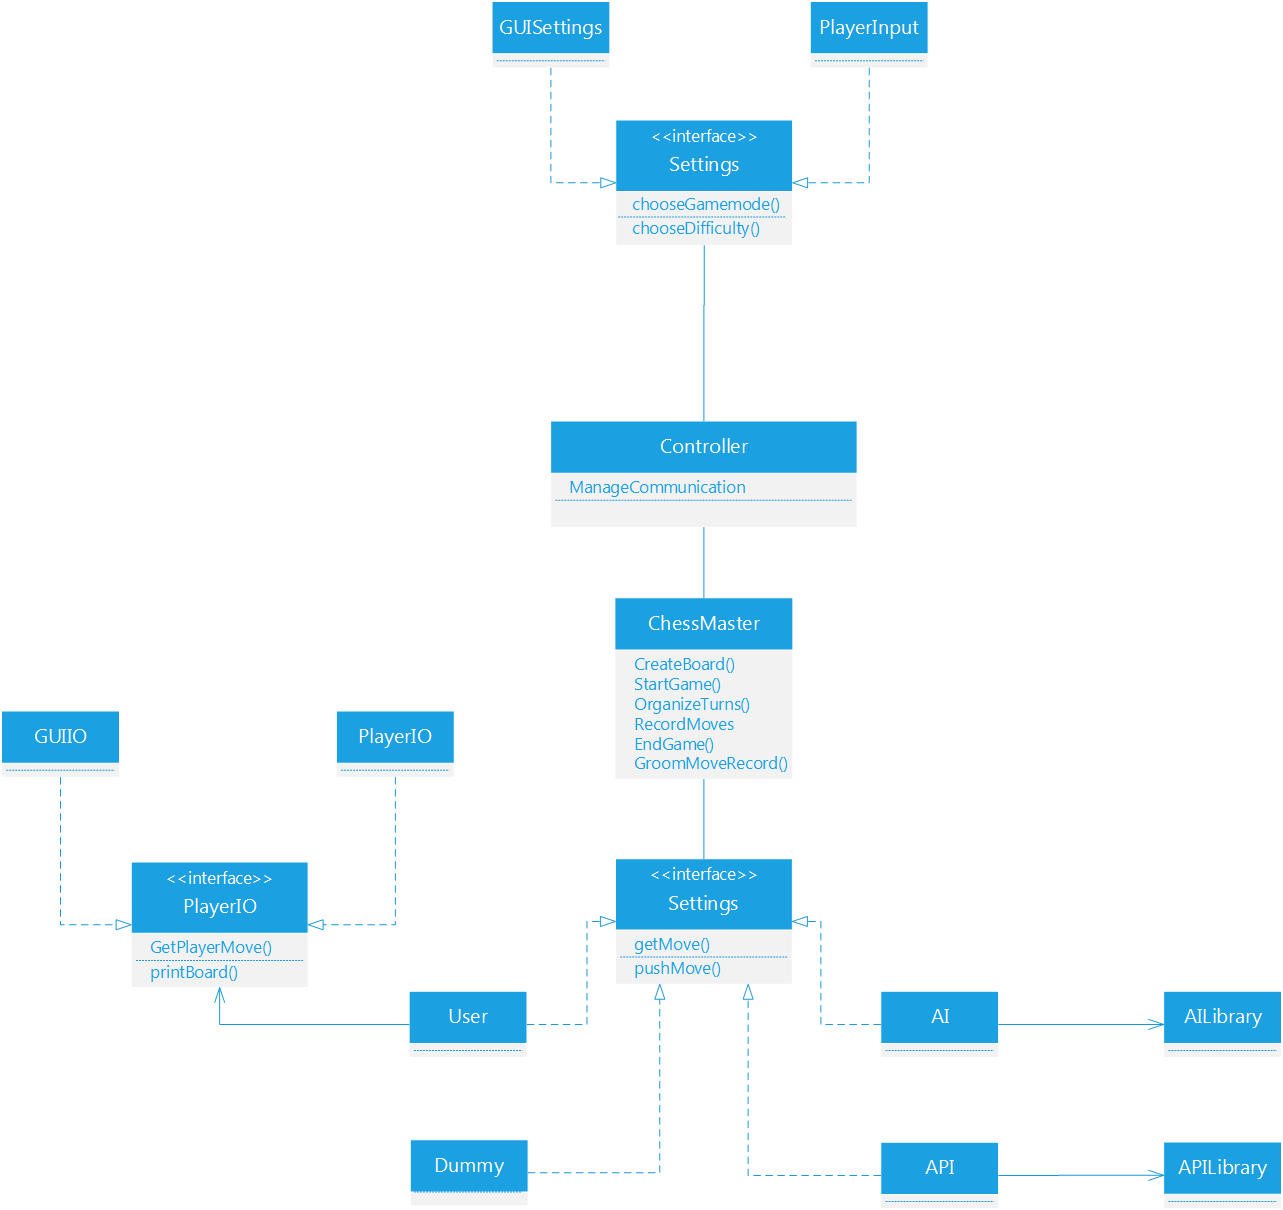
\includegraphics[width=\textwidth*4/5]{images/architecture_class_diagram.png}

\textsuperscript{Figur 3.2.1 Klassendiagramm Architektur ChessAI}
\end{figure}

Als zentrales, Verbindungselement steht zunächst der ``Controller''. Dieser übernimmt die Abfrage aller Optionen, falls diese nicht beim Start des Programms mit übermittelt werden. Zudem initialisiert der Controller die Spielteilnehmer sowie den ``ChessMaster''. Bei letzterem übergibt der Controller diesem die initialisierten Spielteilnehmer. Die Aufgaben des ``ChessMaster'' wird später genauer beschrieben.

Zur Abfrage der Optionen steht dem Controller eine `Settings' Schnittstelle zur Verfügung. Diese wird für Eingaben des Nutzers einerseits über eine Konsole als auch optional über eine grafische Nutzeroberfläche implementiert. Dabei wird abgefragt, welchen Typ die jeweiligen Spielteilnehmer annehmen sollen und es können zudem zusätzliche Optionen für die einzelnen Spieler definiert werden. Als Beispiel kann für Spieler 1 der Typ ``User'' gewählt werden und für Spieler 2 der Typ ``AI''. Dies ermöglicht ein Spiel des Nutzers gegen die im Rahmen dieser Arbeit entwickelte KI. Für die KI wird darauf folgend noch der Schwierigkeitsgrad abgefragt. Zusätzlich kann für jeden Spieler ein Name festgelegt werden.

Die Aufgaben des ``ChessMaster'' erstrecken sich über die Verwaltung des Schachspiels an sich, das Ansprechen der jeweiligen Spieler zum Ermitteln ihrer Züge sowie dem Durchführen des gewählten Spielzugs auf dem Schachbrett. Zusätzlich speichert es jedes Schachbrett, das sich im Laufe des Spiels ergibt, und fügt diese zur ``board\_history.'' Datei hinzu. Diese speichert alle Schachbretter gemeinsam mit einem numerischen Wert. Dieser gibt Aufschluss über Erfolgsaussichten der jeweiligen Akteure des Spiels. Dazu wird nach jedem Spiel zu dem entsprechenden Eintrag in der Datei eine eins zu dem alten Wert aufaddiert, wenn der Spieler der weißen Figuren das Spiel gewonnen hat und eine eins subtrahiert, wenn der Spieler der schwarzen Figuren das Spiel gewonnen hat. Bei einem Unentschieden bleibt der alte Wert bestehen. Dies hilft der KI bei der Bewertung eines Schachbretts unter zur Hilfenahme von statistischen Werten. 

Dieser spricht die vom Controller erstellten Spieler an. Diese können, wie bereits angedeutet, von verschiedenen Typen sein. Zur Auswahl stehen
\begin{itemize}
\item User - Ein menschlicher Akteur kann Züge über eine Nutzerschnittstelle eingeben
\item AI - Die künstliche Intelligenz versucht den best möglichsten Zug zu berechnen
\item Dummy - Ein zufälliger Zug wird ausgewählt
\item (Optional) API - Ein Zug wird über eine Schnittstelle zu einer Online Schachplattform, auf der menschliche sowie künstliche Spieler teilnehmen dürfen, bestimmt
\end{itemize}

Dazu existiert eine ``Player'' Schnittstelle, die für jeden dieser Spieler implementiert werden muss.

Die ``User'' Implementierung greift dabei zur Ermittlung des Zuges auf eine ``PlayerIO'' Schnittstelle zurück. Diese wiederum kann - ähnlich zur ``SettingsUI'' Schnittstelle - sowohl für Eingaben über eine Konsole als auch für Eingaben über eine grafische Nutzeroberfläche implementiert werden.

Die ``AI'' sowie die ``API'' Implementierung greifen für die Ermittlungen ihrer Züge nochmals auf eigens erstellte Bibliotheken zurück, die elementare Funktionen erhalten.

Der genaue Ablauf der Ermittlung der Züge sowie der andere Operationen des Programmes werden in Kapitel \ref{zugfindung-durch-ki}  näher erläutert.

In Figur 3.2.2 ist der sequenteille Ablauf der Funktionsaufrufe erkennbar.

\begin{figure}[h]
\centering
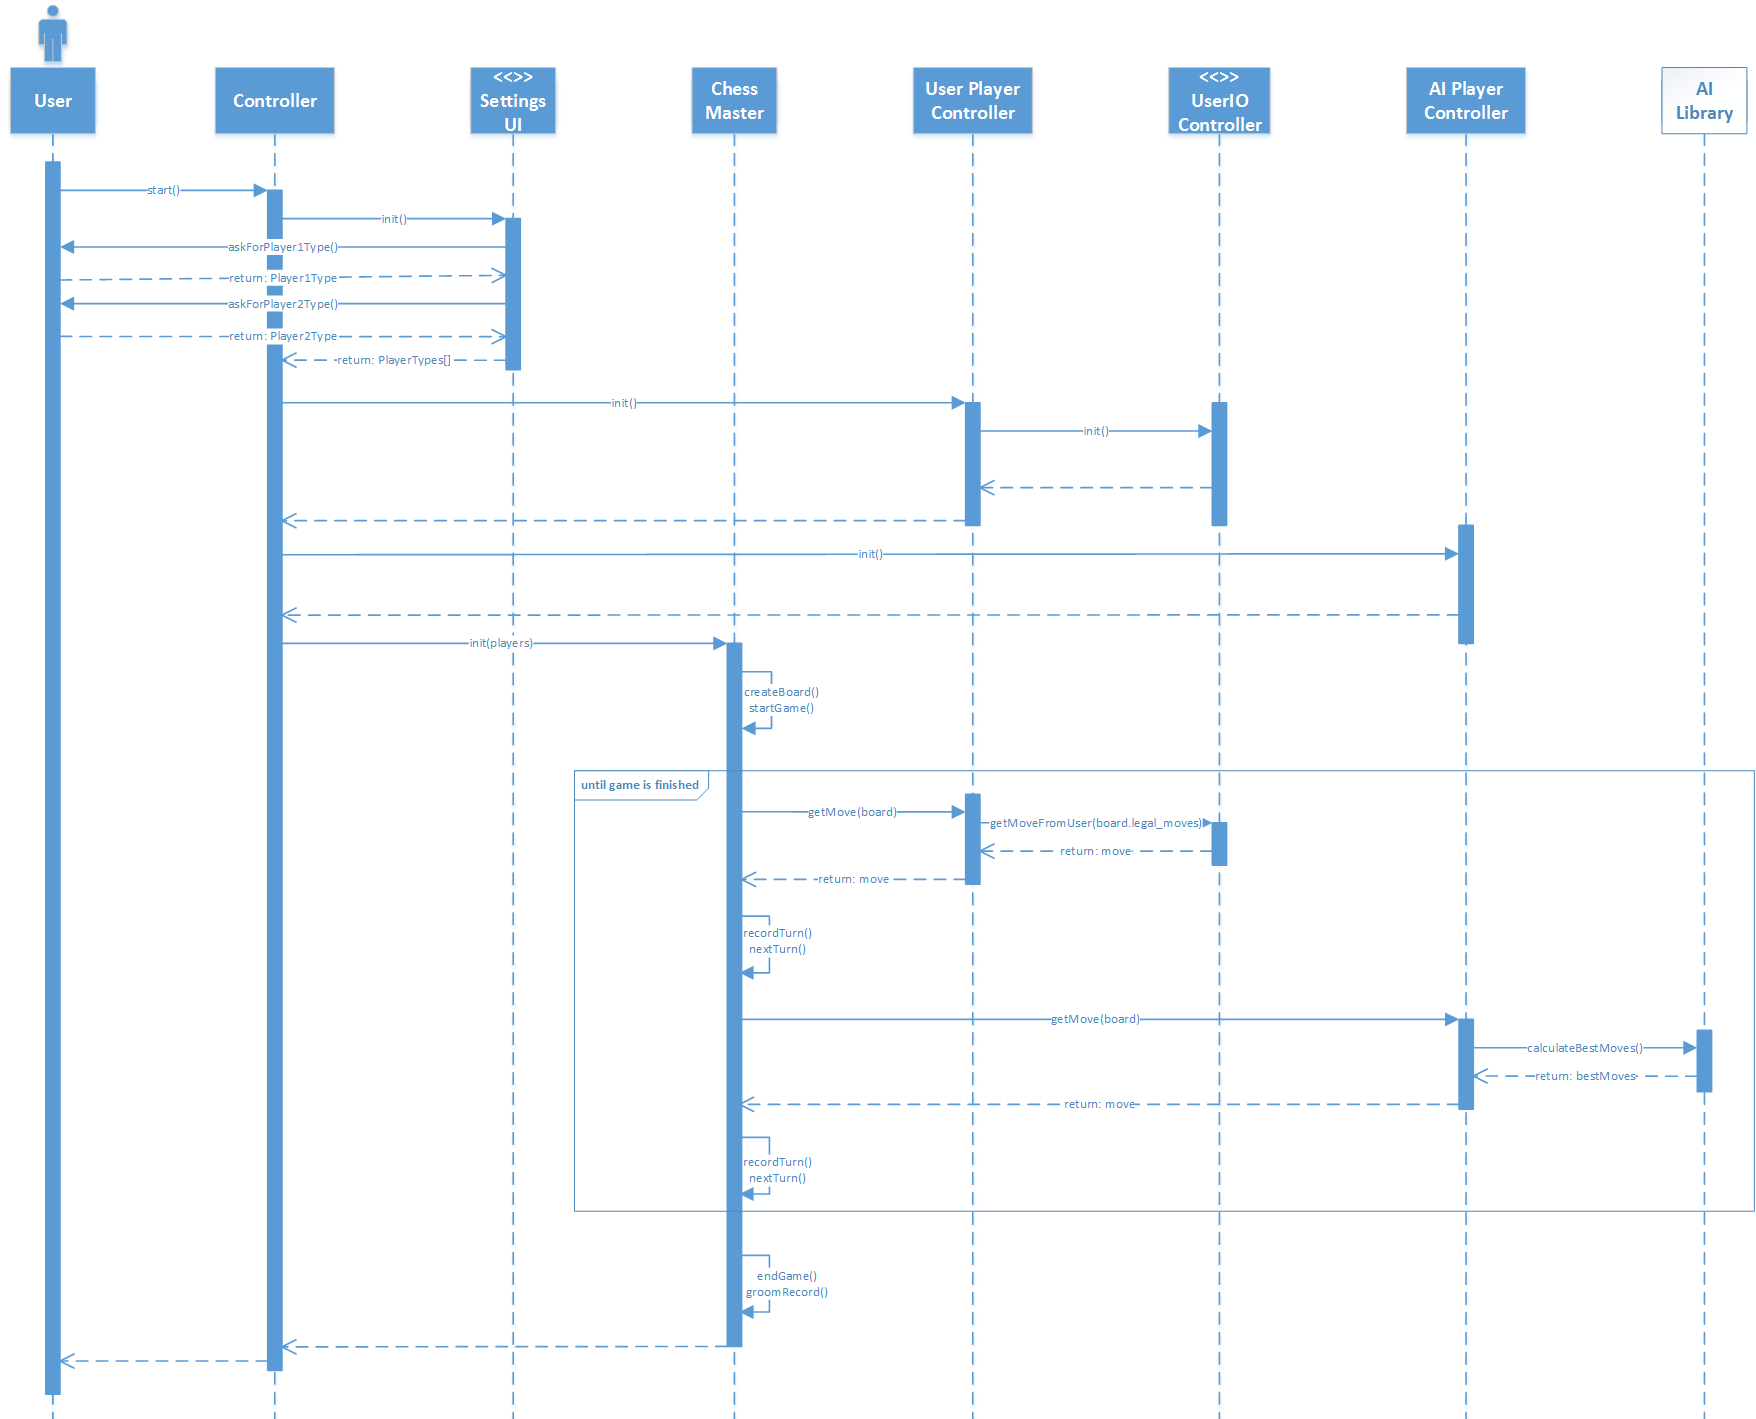
\includegraphics[width=\textwidth]{images/architecture_sequence_diagram.png}

\textsuperscript{Figur 3.2.2 Sequenzdiagramm Architektur ChessAI}
\end{figure}

Dabei wird zunächst über die ``Settings'' Schnittstelle nach den Spielertypen sowie Namen gefragt. initialisiert der ``Controller'' die Spieler, in diesem Fall einerseits den ``User'', der wiederum die ``UserIO'' Schnittstelle implementiert, und außerdem den ``AI'' Player. 

Darauffolgend spricht der ``Controller'' den ``ChessMaster'' an. Dieser startet nun das Spiel und fragt solange wie das Spiel nicht vorbei ist immer abwechselnd erst zu Spieler 1 - dem Nutzer - und dann zu Spieler 2 - der KI - nach dem nächstne Zug. Dabei übergibt der ``ChessMaster'' stets das aktuelle Schachbrett. Der Nutzer ermittelt den durchzuführenden Zug über eine Abfrage an den Nutzer über die entsprechende Schnittstelle, der ``AI'' Spieler, indem dieser Funktionen aus der entsprechenden Bibliothek zur Hilfe nimmt.

Nach jedem Zug fügt der ``ChessMaster'' diesen zum Schachbrett hinzu und speichert dieses in einen Spielverlauf. Nach Ende des Spiels wird dieser in das ``board\_history.csv'' eingepflegt wie weiter oben bei der Beschreibung der Klasse bereits erläutert.

Abschließend beendet der ``ChessMaster'' das Spiel, wenn keine Revanche gewünscht ist, und so wird auch das Programm im Anschluss daran geschlossen.


%TODO: CSV zur Architektur hinzufügen; Funktionsnamen python way
